% Options for packages loaded elsewhere
\PassOptionsToPackage{unicode}{hyperref}
\PassOptionsToPackage{hyphens}{url}
\PassOptionsToPackage{dvipsnames,svgnames,x11names}{xcolor}
%
\documentclass[
  12pt,
  letterpaper,
]{scrreprt}

\usepackage{amsmath,amssymb}
\usepackage{setspace}
\usepackage{iftex}
\ifPDFTeX
  \usepackage[T1]{fontenc}
  \usepackage[utf8]{inputenc}
  \usepackage{textcomp} % provide euro and other symbols
\else % if luatex or xetex
  \usepackage{unicode-math}
  \defaultfontfeatures{Scale=MatchLowercase}
  \defaultfontfeatures[\rmfamily]{Ligatures=TeX,Scale=1}
\fi
\usepackage{lmodern}
\ifPDFTeX\else  
    % xetex/luatex font selection
    \setmainfont[]{Times New Roman}
    \setsansfont[]{Arial}
    \setmonofont[]{Courier New}
\fi
% Use upquote if available, for straight quotes in verbatim environments
\IfFileExists{upquote.sty}{\usepackage{upquote}}{}
\IfFileExists{microtype.sty}{% use microtype if available
  \usepackage[]{microtype}
  \UseMicrotypeSet[protrusion]{basicmath} % disable protrusion for tt fonts
}{}
\usepackage{xcolor}
\usepackage[inner=2.54cm,outer=2.54cm,top=2.54cm,bottom=2.54cm,headsep=22pt,headheight=11pt,footskip=33pt,ignorehead,ignorefoot,heightrounded]{geometry}
\setlength{\emergencystretch}{3em} % prevent overfull lines
\setcounter{secnumdepth}{5}
% Make \paragraph and \subparagraph free-standing
\makeatletter
\ifx\paragraph\undefined\else
  \let\oldparagraph\paragraph
  \renewcommand{\paragraph}{
    \@ifstar
      \xxxParagraphStar
      \xxxParagraphNoStar
  }
  \newcommand{\xxxParagraphStar}[1]{\oldparagraph*{#1}\mbox{}}
  \newcommand{\xxxParagraphNoStar}[1]{\oldparagraph{#1}\mbox{}}
\fi
\ifx\subparagraph\undefined\else
  \let\oldsubparagraph\subparagraph
  \renewcommand{\subparagraph}{
    \@ifstar
      \xxxSubParagraphStar
      \xxxSubParagraphNoStar
  }
  \newcommand{\xxxSubParagraphStar}[1]{\oldsubparagraph*{#1}\mbox{}}
  \newcommand{\xxxSubParagraphNoStar}[1]{\oldsubparagraph{#1}\mbox{}}
\fi
\makeatother


\providecommand{\tightlist}{%
  \setlength{\itemsep}{0pt}\setlength{\parskip}{0pt}}\usepackage{longtable,booktabs,array}
\usepackage{calc} % for calculating minipage widths
% Correct order of tables after \paragraph or \subparagraph
\usepackage{etoolbox}
\makeatletter
\patchcmd\longtable{\par}{\if@noskipsec\mbox{}\fi\par}{}{}
\makeatother
% Allow footnotes in longtable head/foot
\IfFileExists{footnotehyper.sty}{\usepackage{footnotehyper}}{\usepackage{footnote}}
\makesavenoteenv{longtable}
\usepackage{graphicx}
\makeatletter
\newsavebox\pandoc@box
\newcommand*\pandocbounded[1]{% scales image to fit in text height/width
  \sbox\pandoc@box{#1}%
  \Gscale@div\@tempa{\textheight}{\dimexpr\ht\pandoc@box+\dp\pandoc@box\relax}%
  \Gscale@div\@tempb{\linewidth}{\wd\pandoc@box}%
  \ifdim\@tempb\p@<\@tempa\p@\let\@tempa\@tempb\fi% select the smaller of both
  \ifdim\@tempa\p@<\p@\scalebox{\@tempa}{\usebox\pandoc@box}%
  \else\usebox{\pandoc@box}%
  \fi%
}
% Set default figure placement to htbp
\def\fps@figure{htbp}
\makeatother
% definitions for citeproc citations
\NewDocumentCommand\citeproctext{}{}
\NewDocumentCommand\citeproc{mm}{%
  \begingroup\def\citeproctext{#2}\cite{#1}\endgroup}
\makeatletter
 % allow citations to break across lines
 \let\@cite@ofmt\@firstofone
 % avoid brackets around text for \cite:
 \def\@biblabel#1{}
 \def\@cite#1#2{{#1\if@tempswa , #2\fi}}
\makeatother
\newlength{\cslhangindent}
\setlength{\cslhangindent}{1.5em}
\newlength{\csllabelwidth}
\setlength{\csllabelwidth}{3em}
\newenvironment{CSLReferences}[2] % #1 hanging-indent, #2 entry-spacing
 {\begin{list}{}{%
  \setlength{\itemindent}{0pt}
  \setlength{\leftmargin}{0pt}
  \setlength{\parsep}{0pt}
  % turn on hanging indent if param 1 is 1
  \ifodd #1
   \setlength{\leftmargin}{\cslhangindent}
   \setlength{\itemindent}{-1\cslhangindent}
  \fi
  % set entry spacing
  \setlength{\itemsep}{#2\baselineskip}}}
 {\end{list}}
\usepackage{calc}
\newcommand{\CSLBlock}[1]{\hfill\break\parbox[t]{\linewidth}{\strut\ignorespaces#1\strut}}
\newcommand{\CSLLeftMargin}[1]{\parbox[t]{\csllabelwidth}{\strut#1\strut}}
\newcommand{\CSLRightInline}[1]{\parbox[t]{\linewidth - \csllabelwidth}{\strut#1\strut}}
\newcommand{\CSLIndent}[1]{\hspace{\cslhangindent}#1}

\addtokomafont{disposition}{\rmfamily}
\KOMAoptions{chapterprefix=false,appendixprefix=true} %% chapterprefix=true para que aparezca como capitulo 1 o =false para que solo aparezca el numero romano
\KOMAoptions{headings=small}
\raggedright
\setkomafont{pageheadfoot}{\normalfont\normalcolor\footnotesize}
\setkomafont{pagenumber}{\normalfont\normalcolor\footnotesize}
\renewcommand{\thechapter}{\Roman{chapter}}
\renewcommand{\thesection}{\arabic{chapter}.\arabic{section}}
\renewcommand{\thefigure}{\arabic{figure}}
\renewcommand{\thetable}{\arabic{table}}
\renewcommand{\theequation}{\arabic{equation}}
\usepackage{ragged2e}
\justifying
\makeatletter
\@ifpackageloaded{bookmark}{}{\usepackage{bookmark}}
\makeatother
\makeatletter
\@ifpackageloaded{caption}{}{\usepackage{caption}}
\AtBeginDocument{%
\ifdefined\contentsname
  \renewcommand*\contentsname{Tabla de contenidos}
\else
  \newcommand\contentsname{Tabla de contenidos}
\fi
\ifdefined\listfigurename
  \renewcommand*\listfigurename{Índice de figuras}
\else
  \newcommand\listfigurename{Índice de figuras}
\fi
\ifdefined\listtablename
  \renewcommand*\listtablename{Listado de Tablas}
\else
  \newcommand\listtablename{Listado de Tablas}
\fi
\ifdefined\figurename
  \renewcommand*\figurename{Figura}
\else
  \newcommand\figurename{Figura}
\fi
\ifdefined\tablename
  \renewcommand*\tablename{Tabla}
\else
  \newcommand\tablename{Tabla}
\fi
}
\@ifpackageloaded{float}{}{\usepackage{float}}
\floatstyle{ruled}
\@ifundefined{c@chapter}{\newfloat{codelisting}{h}{lop}}{\newfloat{codelisting}{h}{lop}[chapter]}
\floatname{codelisting}{Listado}
\newcommand*\listoflistings{\listof{codelisting}{Listado de Listados}}
\captionsetup{labelsep=colon}
\makeatother
\makeatletter
\makeatother
\makeatletter
\@ifpackageloaded{caption}{}{\usepackage{caption}}
\@ifpackageloaded{subcaption}{}{\usepackage{subcaption}}
\makeatother

\ifLuaTeX
\usepackage[bidi=basic]{babel}
\else
\usepackage[bidi=default]{babel}
\fi
\babelprovide[main,import]{spanish}
\ifPDFTeX
\else
\babelfont{rm}[]{Times New Roman}
\fi
% get rid of language-specific shorthands (see #6817):
\let\LanguageShortHands\languageshorthands
\def\languageshorthands#1{}
\usepackage{bookmark}

\IfFileExists{xurl.sty}{\usepackage{xurl}}{} % add URL line breaks if available
\urlstyle{same} % disable monospaced font for URLs
\hypersetup{
  pdftitle={Unidad de Estadística - UNSAAC},
  pdfauthor={Oscar Chullo Puclla; Betty Alegre Ramos},
  pdflang={es},
  colorlinks=true,
  linkcolor={blue},
  filecolor={Maroon},
  citecolor={Blue},
  urlcolor={Blue},
  pdfcreator={LaTeX via pandoc}}


\title{Unidad de Estadística - UNSAAC}
\author{Oscar Chullo Puclla \and Betty Alegre Ramos}
\date{2024}

\begin{document}
\pagenumbering{roman} %%numeracion en numeros romanos para la primera parte
%% justo hasta antes de indice
\thispagestyle{empty}
\hspace{0.075\textwidth} 
\begin{minipage}[b][\textheight][s]{0.85\textwidth}

%% Formalidad, encabezado nombrev de: U,Facultad,etc
\centering
\textbf{\large{Universidad Nacional de San Antonio Abad del Cusco}} \\
\textbf{\large{Facultad de ciencias físicas, químicas y matemáticas}} \\
\textbf{\large{Escuela profesional de matemáticas y estadística}} \\
\textbf{\large{}} \\ %% subtitle es para nominación del año
\vspace{1\baselineskip}

%% Logo central

\includegraphics[width=6cm]{imagen/unsaac.png}
\vspace{1\baselineskip}

% Parte tesis encuadrada
\Large{\textbf{INFORME DE PRÁCTICAS PRE-PROFESIONALES:}} \\
\hrulefill \\
{\Large\bfseries{Unidad de Estadística - UNSAAC}} \\
\hrulefill 

% Abstract


\large{
\flushleft \hspace{6cm}
\textbf{JEFE DE LA UNIDAD DE} \\\hspace{6cm}
\textbf{ESTADÍSTICA:} \\
\hspace{6cm} Econ. Carlos Huamán Aguilar \\ 
\smallskip
\hspace{6cm} \textbf{PRESENTADO POR:} \\ \hspace{6cm}
 {\large{Oscar Chullo Puclla}}
\\
\smallskip
\hspace{6cm} \textbf{DOCENTE:} \\ \hspace{6cm}
%
{\large{Betty Alegre Ramos}}%

}

\vfill

\centering
\Large{CUSCO - PERÚ} \\
\Large{2024}
\vspace{0.1\textheight} 
\end{minipage}

%%% Colocar capitulo y pagina sobre el índice
\addtocontents{toc}{\hspace{-0.1mm} \textbf{Capítulos}}
\addtocontents{toc}{\hfill \textbf{Página} \par}
\addtocontents{toc}{\vspace{-2mm} \hspace{-7.5mm} \hrule \par}

%%% Editar dedicatoria

\pagebreak %% no quitar porque se juntara todo

%% Editar agradecimiento

\setlength{\parindent}{1.5em}

\renewcommand*\contentsname{Índice general}
{
\hypersetup{linkcolor=}
\setcounter{tocdepth}{2}
\tableofcontents
}
\listoffigures

\setstretch{2}
\bookmarksetup{startatroot}

\chapter{Introducción}\label{introducciuxf3n}

\pagenumbering{arabic}

Las prácticas pre-profesionales nos permiten integrar los conocimientos
y habilidades adquiridas en la formación académica, puesto que estas
constituyen una fase clave en el desarrollo profesional. En este
contexto, se ha tenido la oportunidad de realizar Prácticas
Pre-Profesionales (PPP) en la Universidad Nacional de San Antonio Abad
del Cusco, en particular en la Unidad de Estadística.

Esta oficina se encuentra ubicada en el pabellón del instituto de
idiomas, tercer piso, las prácticas se desarrollaron durante cinco horas
diarias, de 8:00 a.m. a 1:00 p.m. El periodo de tiempo establecido fue
de cuatro meses, se desarrolló diversas actividades durante este periodo
resaltándose los estadísticos para el compendio estadístico 2024, el
costo financiero por alumno 2019-2023 y la organización de bases de
datos

El presente informe ofrece un relato detallado de las funciones
desempeñadas durante el periodo de las prácticas pre-profesionales.

\bookmarksetup{startatroot}

\chapter{Unidad de Estadística}\label{unidad-de-estaduxedstica}

La Unidad de Estadística es una Unidad Orgánica comprendida dentro de la
organización de la Direccion de Sistemas de Informacion, tiene a su
cargo la recopilación, sistematización, análisis y publicación de los
datos estadísticos necesarios para la planificación y programación de
las actividades que desarrolla la universidad, realiza estudios y
diagnósticos sociales, económicos y académicos.(Estadística, 2024)

\section{Funciones}\label{funciones}

\begin{itemize}
\tightlist
\item
  Ejecutar las actividades estadísticas de acuerdo a los requerimientos
  institucionales.
\item
  Capturar, elaborar, revisar, criticar validar y procesar para su
  difusión, las estadísticas a fin de facilitar la gestión y toma de
  decisiones.
\item
  Suministrar datos estadísticos solicitados por las diferentes
  dependencias del Nivel Nacional, Regional, Local e institucional.
\item
  Asesorar a la Alta Dirección en asuntos de manejo de información
  estadística.
\item
  Realizar estudios estadísticos sobre aspectos diversos de la
  problemática universitaria que permita un mejor conocimiento de la
  realidad.
\item
  Elaborar indicadores e índices económicos y sociales para el análisis
  y formulación de políticas institucionales.
\item
  Establecer métodos para el cálculo de tendencias y/o proyecciones
  estadísticas.
\item
  Realizar diagnósticos sociales económicos y académicos de la
  Universidad.
\item
  Publicar anualmente boletines estadísticos, trípticos y otros
  documentos.
\item
  Organizar y administrar el banco de datos estadísticos de la
  institución.
\item
  Velar por la capacitación permanente del personal del Área.
\item
  Elaborar el plan de trabajo anual del Área.
\item
  Coordinar la recopilación, procesamiento de datos estadísticos con las
  diferentes dependencias de la institución.
\end{itemize}

\section{Organización}\label{organizaciuxf3n}

\begin{enumerate}
\def\labelenumi{\arabic{enumi}.}
\tightlist
\item
  \textbf{Órgano de Dirección:} ``Unidad de Estadística''
\end{enumerate}

\begin{itemize}
\tightlist
\item
  \textbf{Órganos de Línea:} ``Unidad de Recopilación, procesamiento y
  análisis estadístico'' y ``Unidad de Estudios socio económicos''
\end{itemize}

\begin{enumerate}
\def\labelenumi{\arabic{enumi}.}
\setcounter{enumi}{1}
\tightlist
\item
  \textbf{Personal del Área:}
\end{enumerate}

\begin{itemize}
\tightlist
\item
  \textbf{Jefe de la Unidad de Estadística:} Econ CARLOS HUAMAN AGUILAR
\item
  \textbf{Teléfono:} 989414939
\item
  \textbf{Anexo:} 1004,
\item
  \textbf{correo electrónico:} estadistica@unsaac.edu.pe
\end{itemize}

\section{Misión}\label{misiuxf3n}

Producir y difundir las estadísticas de la UNSAAC con calidad y
transparencia para la toma de decisiones en materia académica,
administrativa y política institucional.

\section{Visión}\label{visiuxf3n}

Ser reconocida, como la fuente fundamental de las estadísticas de la
UNSAAC por la calidad en sus productos y servicios ofrecidos a los
demandantes.

\bookmarksetup{startatroot}

\chapter{Desarrollo de Prácticas Pre-Profesionales
(PPP)}\label{desarrollo-de-pruxe1cticas-pre-profesionales-ppp}

\section{Setiembre}\label{setiembre}

\subsection{Elaboracion del registro de bachilleres y titulados de la
escuela profesional de Ingeniería Informática y de Sistemas
(1993-2023)}\label{elaboracion-del-registro-de-bachilleres-y-titulados-de-la-escuela-profesional-de-ingenieruxeda-informuxe1tica-y-de-sistemas-1993-2023}

La primera actividad realizada fue la de elaborar un registro completo
de bachilleres y titulados de la E.P. de Ingeniería Informática y de
Sistemas, durante el periodo 1993-2023 bajo solicitud del Director de
escuela correspondiente, se hizo una revision de recursos dentro de la
Unidad de Estadística en los cuales se evidenciaron las siguientes
dificultades: - Falta de Organización en los documentos y la información
de años pasados. - Pérdida de Información de los registros
correspondientes al año 2007, no hubo en libros ni en los CD´s.

Por ello se remitió un registro del periodo 1993-2023 a excepción del
2007.

\subsection{Elaboración de estadísticos de los estudiantes matriculados
del semestre
2024-I}\label{elaboraciuxf3n-de-estaduxedsticos-de-los-estudiantes-matriculados-del-semestre-2024-i}

Se realizo una limpieza de datos en el registro de estudiantes
matriculados correspondientes al semestre 2024-I, puesto que se tenia
error en el registro de sexo (varones registrados como mujeres y
viceversa), e información faltante en los lugares de procedencia, años
de nacimiento y edades, recurriendose al uso de tecnicas de imputación
de datos adquiridos en la formación como estadístico. A continuación se
presentan los resultados obtenidos en grafícos:

\begin{figure}[H]

\caption{Alumnos matriculados según sexo, semestre 2024-I}

{\centering \includegraphics[width=0.7\linewidth,height=\textheight,keepaspectratio]{imagen/imagen3.png}

}

\end{figure}%%
\begin{figure}[H]

\caption{Alumnos matriculados según facultad, semestre 2024-I}

{\centering \includegraphics[width=0.6\linewidth,height=\textheight,keepaspectratio]{imagen/imagen5.png}

}

\end{figure}%%
\begin{figure}[H]

\caption{Alumnos matriculados según facultad y sexo, semestre 2024-I}

{\centering \pandocbounded{\includegraphics[keepaspectratio]{imagen/imagen4.png}}

}

\end{figure}%%
\begin{figure}[H]

\caption{Alumnos matriculados según escuelas profesionales, semestre
2024-I}

{\centering \pandocbounded{\includegraphics[keepaspectratio]{imagen/imagen2.png}}

}

\end{figure}%%
\begin{figure}[H]

\caption{Alumnos matriculados por escuelas profesionales y sexo,
semestre 2024-I}

{\centering \pandocbounded{\includegraphics[keepaspectratio]{imagen/imagen1.png}}

}

\end{figure}%%
\begin{figure}[H]

\caption{Alumnos matriculados según región de procedencia, semestre
2024-I}

{\centering \includegraphics[width=0.6\linewidth,height=\textheight,keepaspectratio]{imagen/imagen6.png}

}

\end{figure}%%
\begin{figure}[H]

\caption{Alumnos matriculados de la región Cusco, semestre 2024-I}

{\centering \includegraphics[width=0.6\linewidth,height=\textheight,keepaspectratio]{imagen/imagen8.png}

}

\end{figure}%%
\begin{figure}[H]

\caption{Alumnos matriculados de la provincia del Cusco, semestre
2024-I}

{\centering \includegraphics[width=0.6\linewidth,height=\textheight,keepaspectratio]{imagen/imagen7.png}

}

\end{figure}%%
\begin{figure}[H]

\caption{Alumnos matriculados por edad, semestre 2024-I}

{\centering \includegraphics[width=0.8\linewidth,height=\textheight,keepaspectratio]{imagen/imagen9.png}

}

\end{figure}%

\section{Octubre}\label{octubre}

\subsection{Elaboración del registro de beneficiarios del comedor
universitario (2023-I, 2023-II y
2024-I)}\label{elaboraciuxf3n-del-registro-de-beneficiarios-del-comedor-universitario-2023-i-2023-ii-y-2024-i}

Se tuvo una solicitud del rectorado en el que se pedia una elaboración
del registro de estudiantes beneficiarios, es decir un registro que
cuente las siguientes características: - Estudiantes organizados por
escuela profesional - Veces en la que un estudiante ha reservado cupo -
Veces en la que el estudiante ha hecho uso del comedor en un cupo

A continuación se muestran los primeros datos de dicho registro

\begin{figure}[H]

\caption{Registro de beneficiarios del comedor universitario (2023-I,
2023-II y 2024-I)}

{\centering \pandocbounded{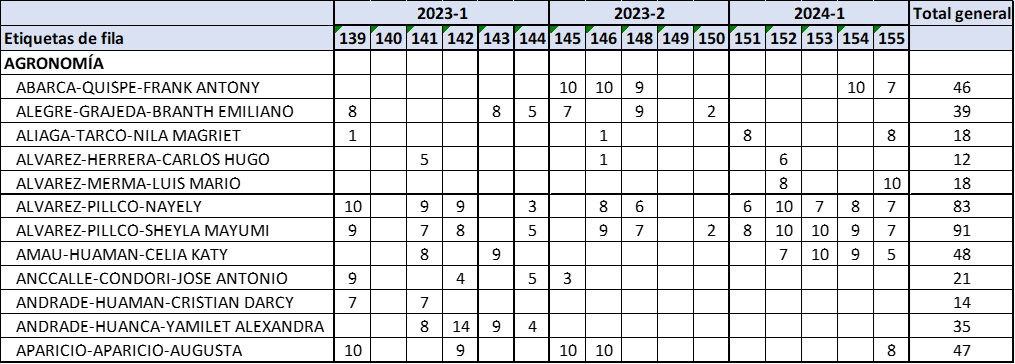
\includegraphics[keepaspectratio]{imagen/cuadro1.png}}

}

\end{figure}%

\subsection{Elaboración del registro de becados beneficiarios del
comedor universitario (2023-I, 2023-II y
2024-I)}\label{elaboraciuxf3n-del-registro-de-becados-beneficiarios-del-comedor-universitario-2023-i-2023-ii-y-2024-i}

En la segunda parte de la solicitud, se disponia elaborar un registro
para los becados beneficiarios del comedor, con el objetivo d
eidentificar a la población que hacia uso del beneficio y la que no mlo
hacia para establecer nuevos filtros en la selección de beneficiarios
del comedor universitario, para los cuales se tuvo las siguientes
características:

\begin{itemize}
\tightlist
\item
  Estudiantes organizados por escuela profesional
\item
  Veces en la que el estudiante ha hecho uso del comedor en un cupo
\end{itemize}

\begin{figure}[H]

\caption{Registro de becarios beneficiarios del comedor universitario
(2023-I, 2023-II y 2024-I)}

{\centering \pandocbounded{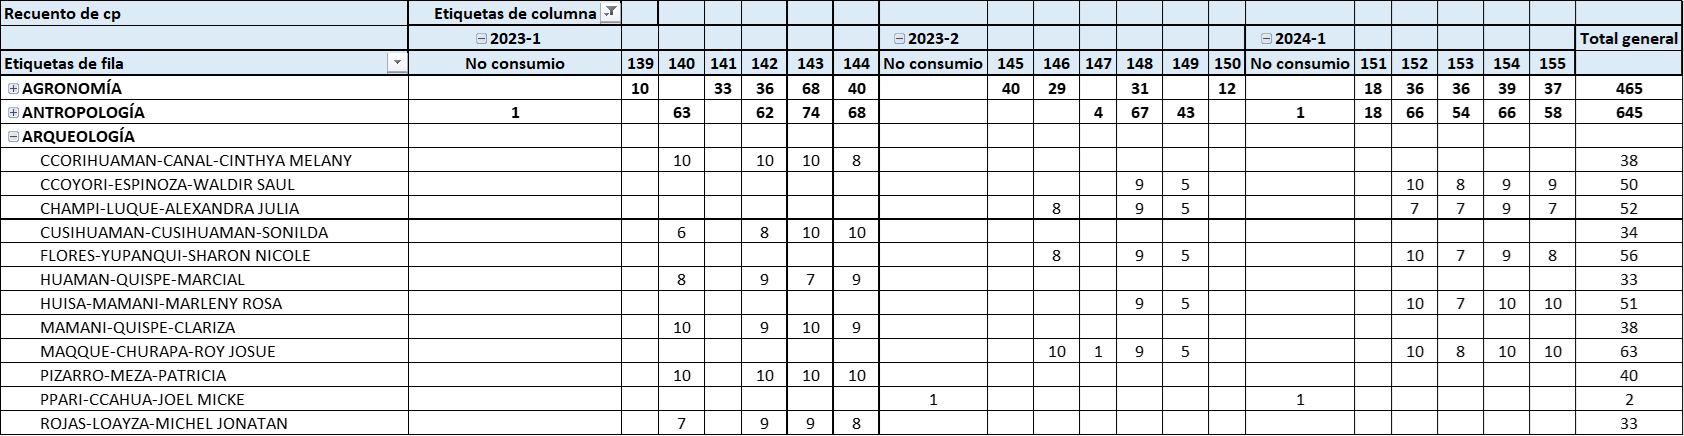
\includegraphics[keepaspectratio]{imagen/cuadro2.png}}

}

\end{figure}%

\subsection{Elaboración de estadísticos de los docentes nombrados en el
semestre
2024-I}\label{elaboraciuxf3n-de-estaduxedsticos-de-los-docentes-nombrados-en-el-semestre-2024-i}

Se tuvo la base de datos de los docentes nombrados que ejercieron su
profesión en el semestre académico 2024-I, para el cual se realizaron
los estadísticos correspondientes según el compendio estadístico,
obteniéndose los siguientes resultados:

\begin{figure}[H]

\caption{Docentes nombrados según sexo, semestre 2024-I}

{\centering \pandocbounded{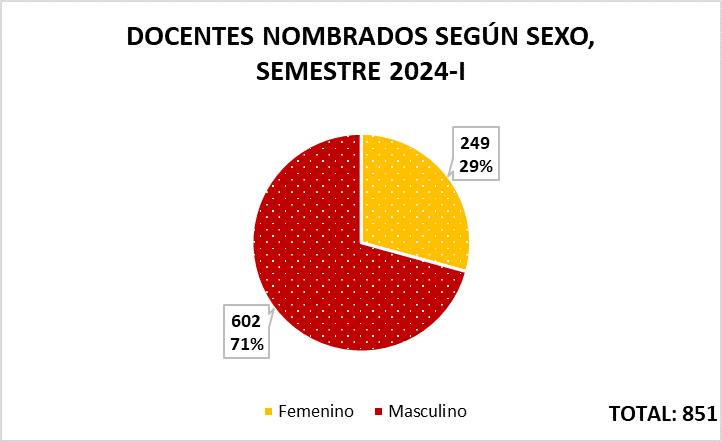
\includegraphics[keepaspectratio]{imagen/sao.png}}

}

\end{figure}%%
\begin{figure}[H]

\caption{Docentes nombrados según departamento académico y sexo,
semestre 2024-I}

{\centering \pandocbounded{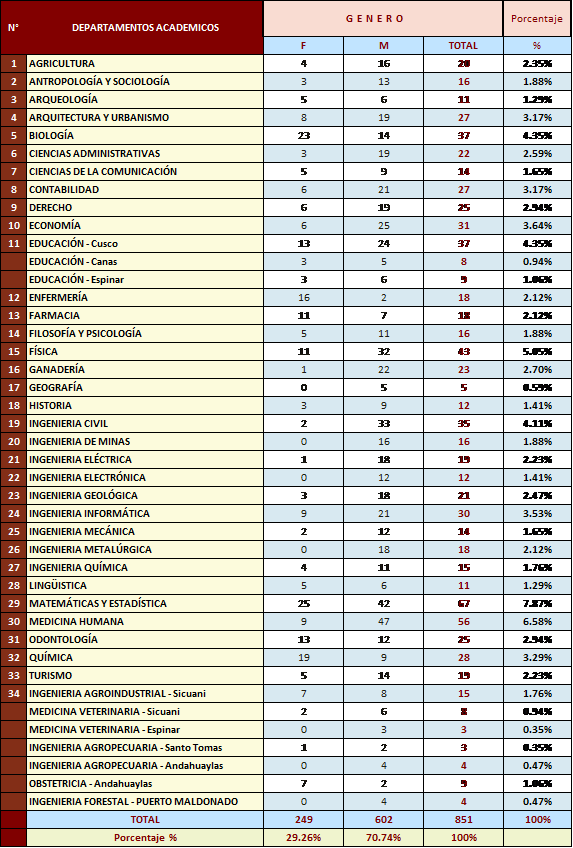
\includegraphics[keepaspectratio]{imagen/sao1.png}}

}

\end{figure}%%
\begin{figure}[H]

\caption{Docentes nombrados según facultad y departamento académico,
semestre 2024-I}

{\centering \pandocbounded{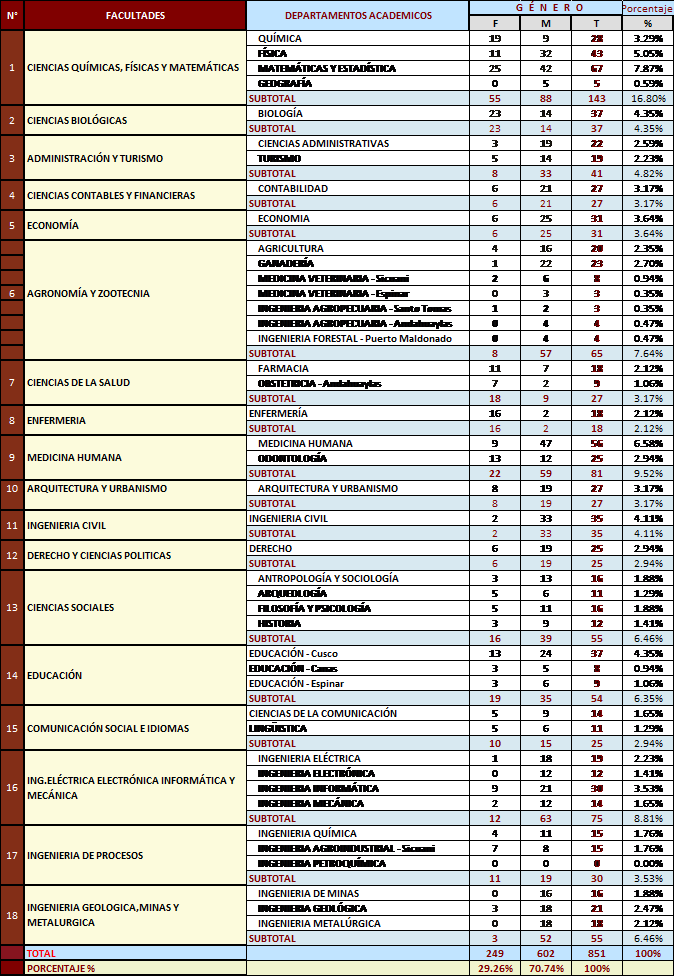
\includegraphics[keepaspectratio]{imagen/sao2.png}}

}

\end{figure}%%
\begin{figure}[H]

\caption{Docentes nombrados según nivel académico alcanzado, semestre
2024-I}

{\centering \pandocbounded{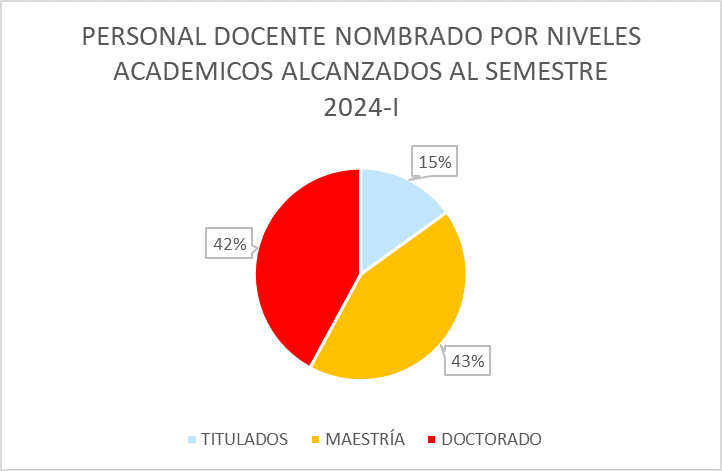
\includegraphics[keepaspectratio]{imagen/sao3.png}}

}

\end{figure}%%
\begin{figure}[H]

\caption{Docentes nombrados según nivel académico alcanzado al semestre
2024-I}

{\centering \pandocbounded{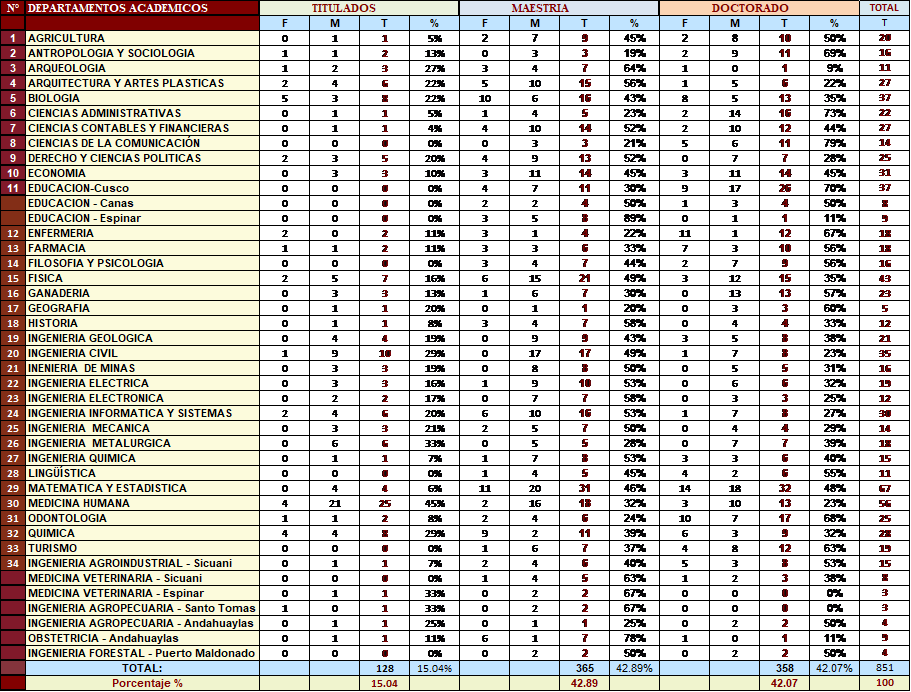
\includegraphics[keepaspectratio]{imagen/sao4.png}}

}

\end{figure}%%
\begin{figure}[H]

\caption{Docentes nombrados según categoría y dedicación por
departamento académico y sexo, semestre 2024-I}

{\centering \pandocbounded{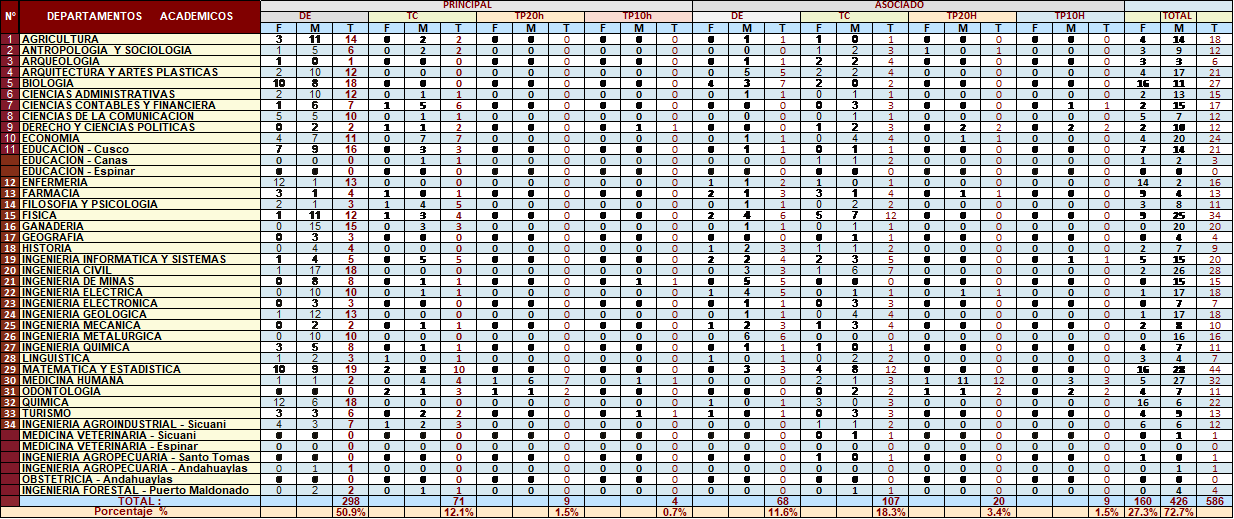
\includegraphics[keepaspectratio]{imagen/sao5.png}}

}

\end{figure}%%
\begin{figure}[H]

\caption{Docentes nombrados según categoría y dedicación por
departamento académico y sexo; semestre 2024-I}

{\centering \pandocbounded{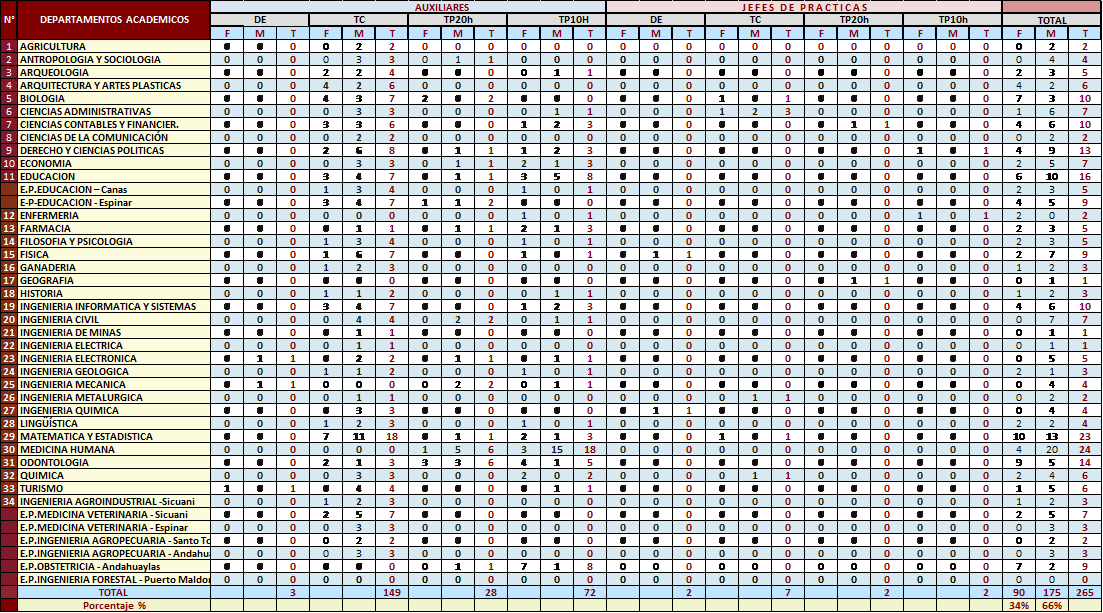
\includegraphics[keepaspectratio]{imagen/sao6.png}}

}

\end{figure}%%
\begin{figure}[H]

\caption{Docentes nombrados según categoría y dedicación, semestre
2024-I}

{\centering \pandocbounded{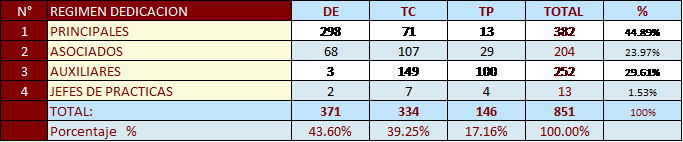
\includegraphics[keepaspectratio]{imagen/sao7.png}}

}

\end{figure}%

\subsection{Revisión de ``Variables universitarias 2019-2023 y
proyecciones estadísticas
2024-2028''}\label{revisiuxf3n-de-variables-universitarias-2019-2023-y-proyecciones-estaduxedsticas-2024-2028}

Se tenia el archivo de ``Variables universitarias 2019-2023 y
proyecciones estadísticas 2024-2028'', sin embargo se tuvieron algunos
errores en la redacción y organización de dicho documento, por lo que se
hizo una revisión detallada para la levantación de observaciones,
posterior a la revisión se realizo la publicacion del documento al cual
puede accederse mediante el siguiente link:
https://drive.google.com/file/d/1aFfQPyAojehU2Fm-d6QCdIGCR4-4VPjz/view

\subsection{Elaboracion de estadísticos de presupuesto
2019-2023}\label{elaboracion-de-estaduxedsticos-de-presupuesto-2019-2023}

Se inició con la elaboración de estadísticos de presupuesto 2019-2023,
en los que se describe el presupuesto autorizado, ejecutado y el saldo
restante, según asignaciones genéricas entre recursos ordinarios y
recursos directamente recaudados, en este mes se realizo lo
correspondiente al año 2019.

\subsection{Revisión del informe de graduados y titulados
2023}\label{revisiuxf3n-del-informe-de-graduados-y-titulados-2023}

Se hizo una revisión del informe de graduados y titulados, de los cuales
se ha contrastado las bases de datos para realizar el registro completo
de graduados y titulados del 2023, para este registro se utilizo la base
de datos de años anteriores como datos para complementar los datos
faltantes en el informe

\section{Noviembre}\label{noviembre}

\subsection{Elaboracion de estadísticos de presupuesto
2019-2023}\label{elaboracion-de-estaduxedsticos-de-presupuesto-2019-2023-1}

Se continuó con la elaboración de estadísticos de presupuesto 2019-2023,
en los que se describe el presupuesto autorizado, ejecutado y el saldo
restante, según asignaciones genéricas entre recursos ordinarios y
recursos directamente recaudados, en este mes se realizo lo faltante y
se completaron los estadísticos, véase uno de los cuadros a
continuación:

\begin{figure}[H]

\caption{Presupuesto Total ejecutado entre Recursos Ordinarios y
Recursos Directamente Recaudados 2019 - Servicios Adecuados de Apoyo al
Estudiante (Bienestar y Asistencia Social)}

{\centering \pandocbounded{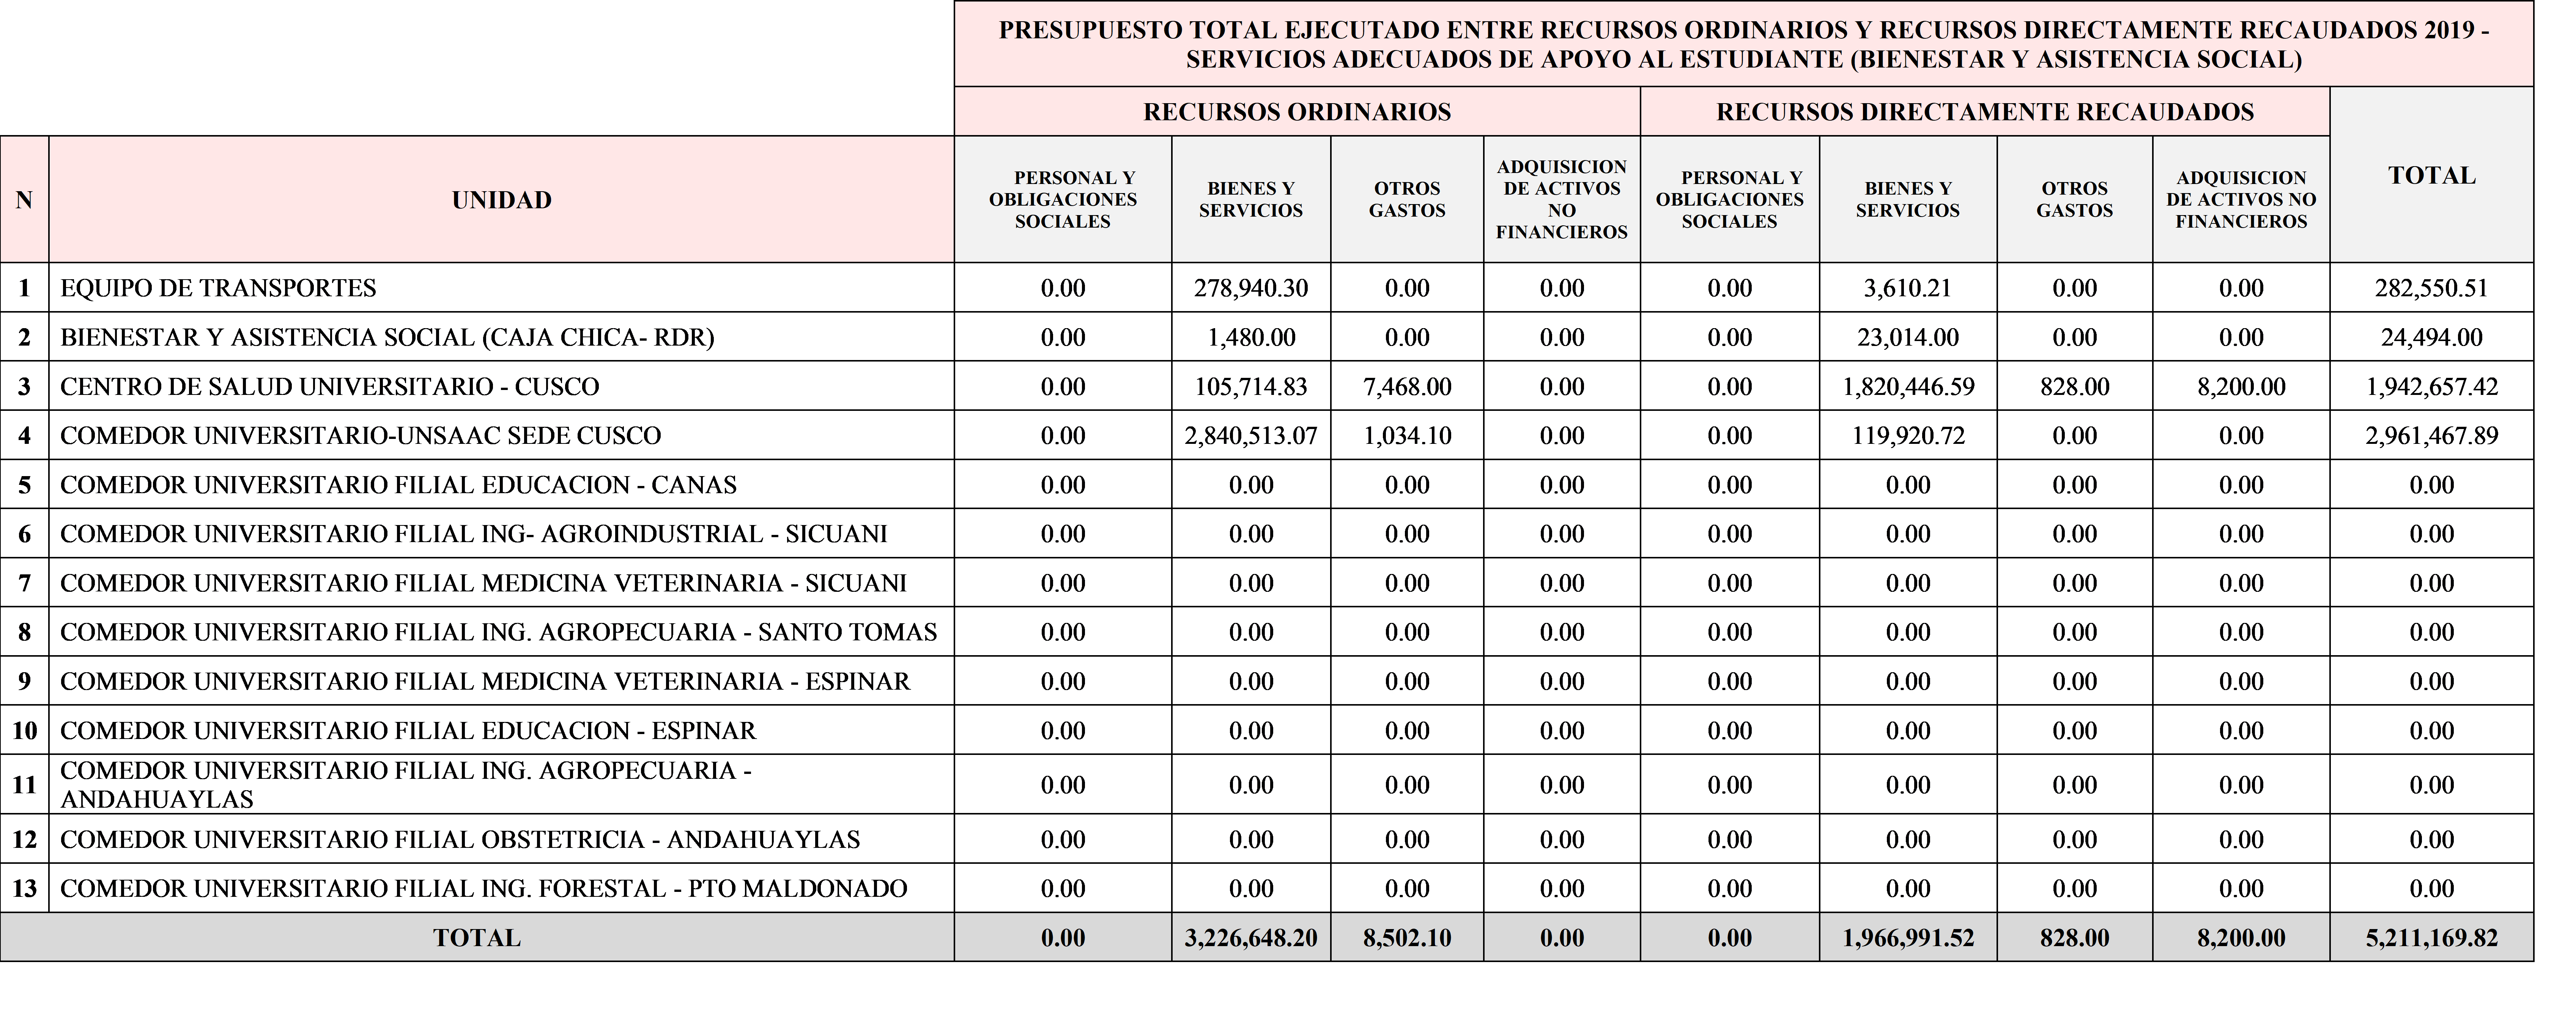
\includegraphics[keepaspectratio]{imagen/eje1.png}}

}

\end{figure}%

Se realizaron series por asignación genérica con respecto al presupuesto
ejecutado, a continuación se muestra una de las series realizadas:

\begin{figure}[H]

\caption{Tabla de Presupuesto Total ejecutado 2019-2023}

{\centering \pandocbounded{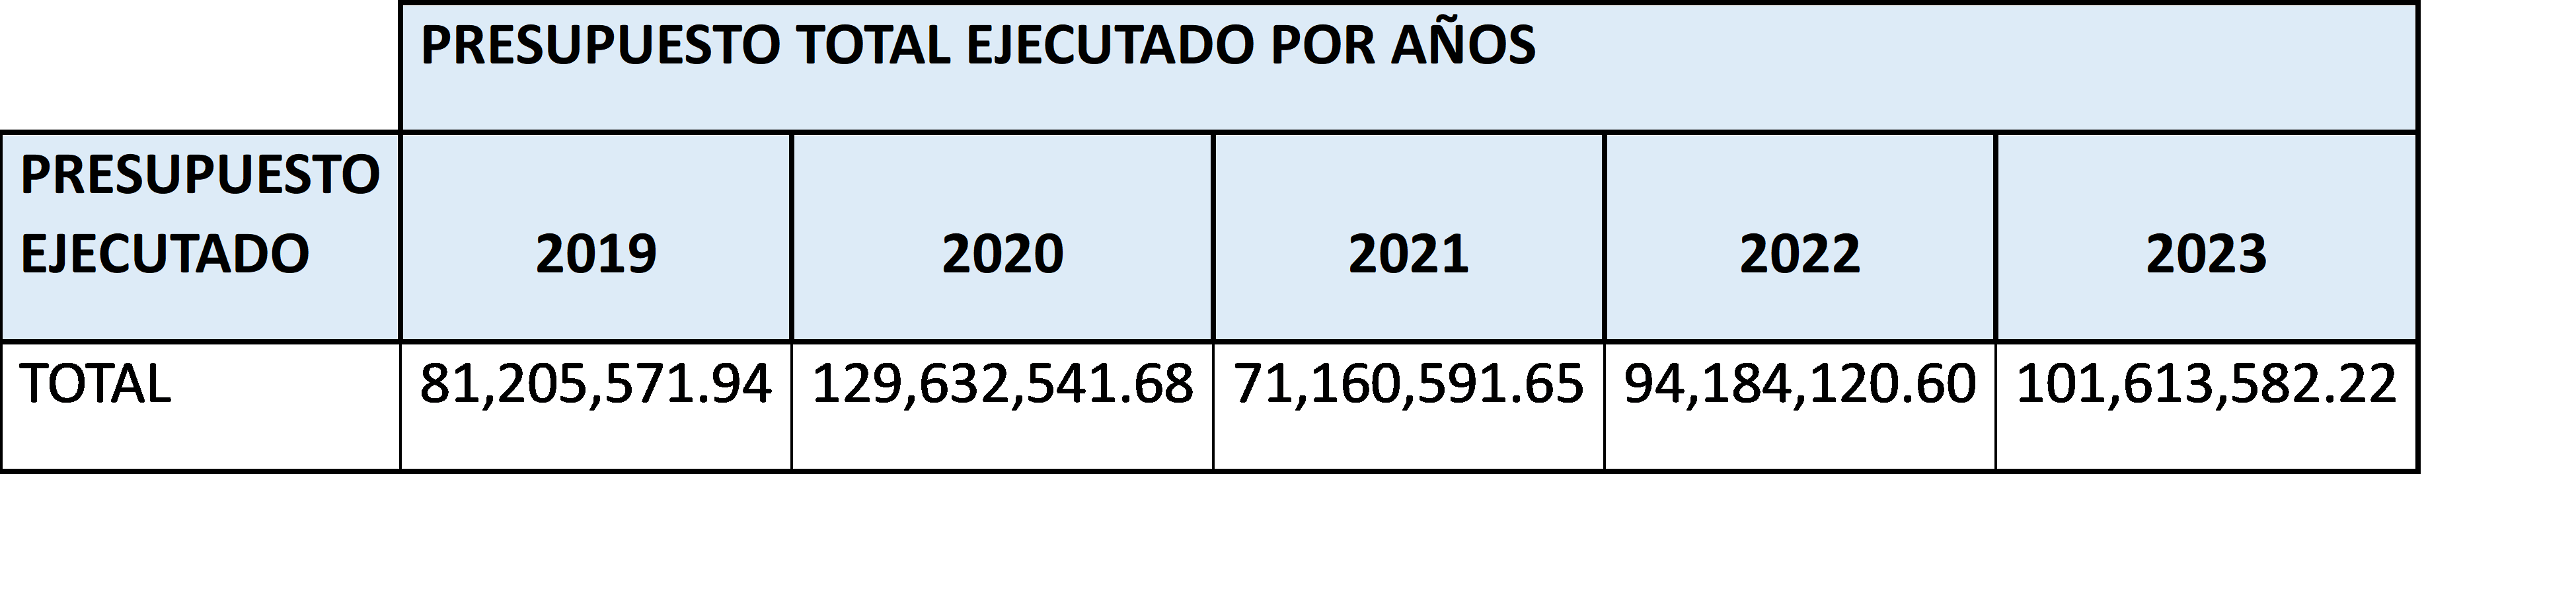
\includegraphics[keepaspectratio]{imagen/pres.png}}

}

\end{figure}%%
\begin{figure}[H]

\caption{Figura de Presupuesto Total ejecutado 2019-2023}

{\centering \pandocbounded{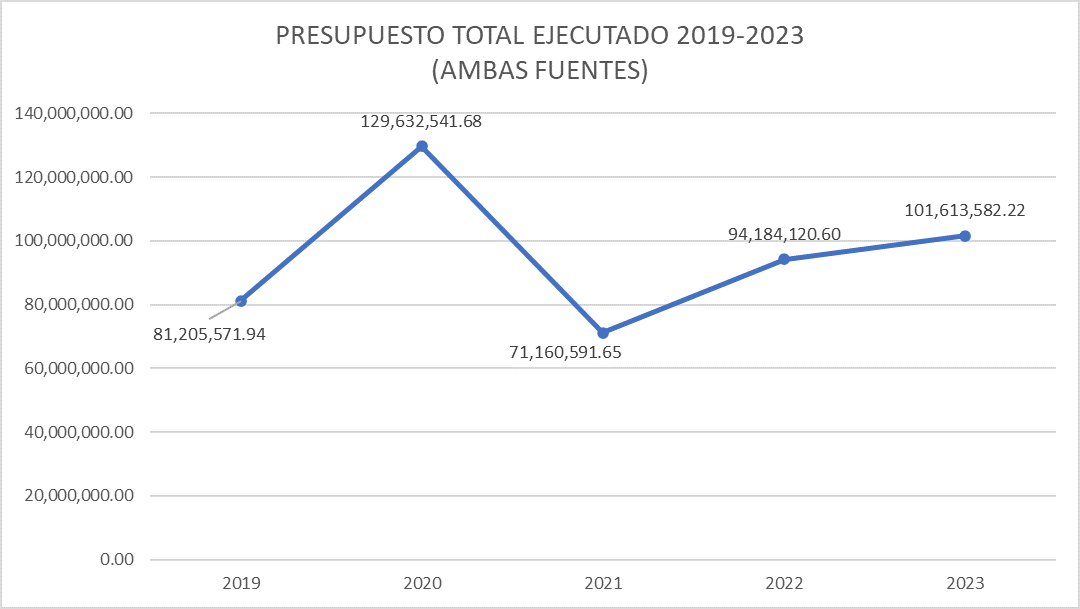
\includegraphics[keepaspectratio]{imagen/pres1.png}}

}

\end{figure}%

\subsection{Instalación de R y
Python}\label{instalaciuxf3n-de-r-y-python}

Realizando una visión al futuro se hizo la instalación de los software R
(Rmarkdown + quarto) y Python (Anaconda Navigator) y LaTeX para el
analisis de datos estadísticos mediante la programación y el machine
learning.

En esta sección se trabajo en una guia en HTML para nuevos usuarios de
R, Rmarkdown y quarto, el cual fue publicado en RPubs, al cual puede
accederse con el siguiente enlace:
https://rpubs.com/Oscar\_ChulloP/installR

\subsection{Elaboracion de estadísticos de presupuesto 2019-2023: Costo
por
estudiante}\label{elaboracion-de-estaduxedsticos-de-presupuesto-2019-2023-costo-por-estudiante}

Luego de la entrega de los estadísticos de presupuesto, se llegó a un
acuerdo de elaborar estadísticos de gasto financiero o costo por alumno,
los cuales siguieron los lineamientos de una estructura de años
anteriores, a continuación se presenta los cuadros de gasto:

\begin{figure}[H]

\caption{Presupuesto total ejecutado por escuela profesional 2019-2023}

{\centering \pandocbounded{
\includegraphics[keepaspectratio]{imagen/cost1.png}}

}

\end{figure}%%
\begin{figure}[H]

\caption{Costo por alumno, 2019}

{\centering \pandocbounded{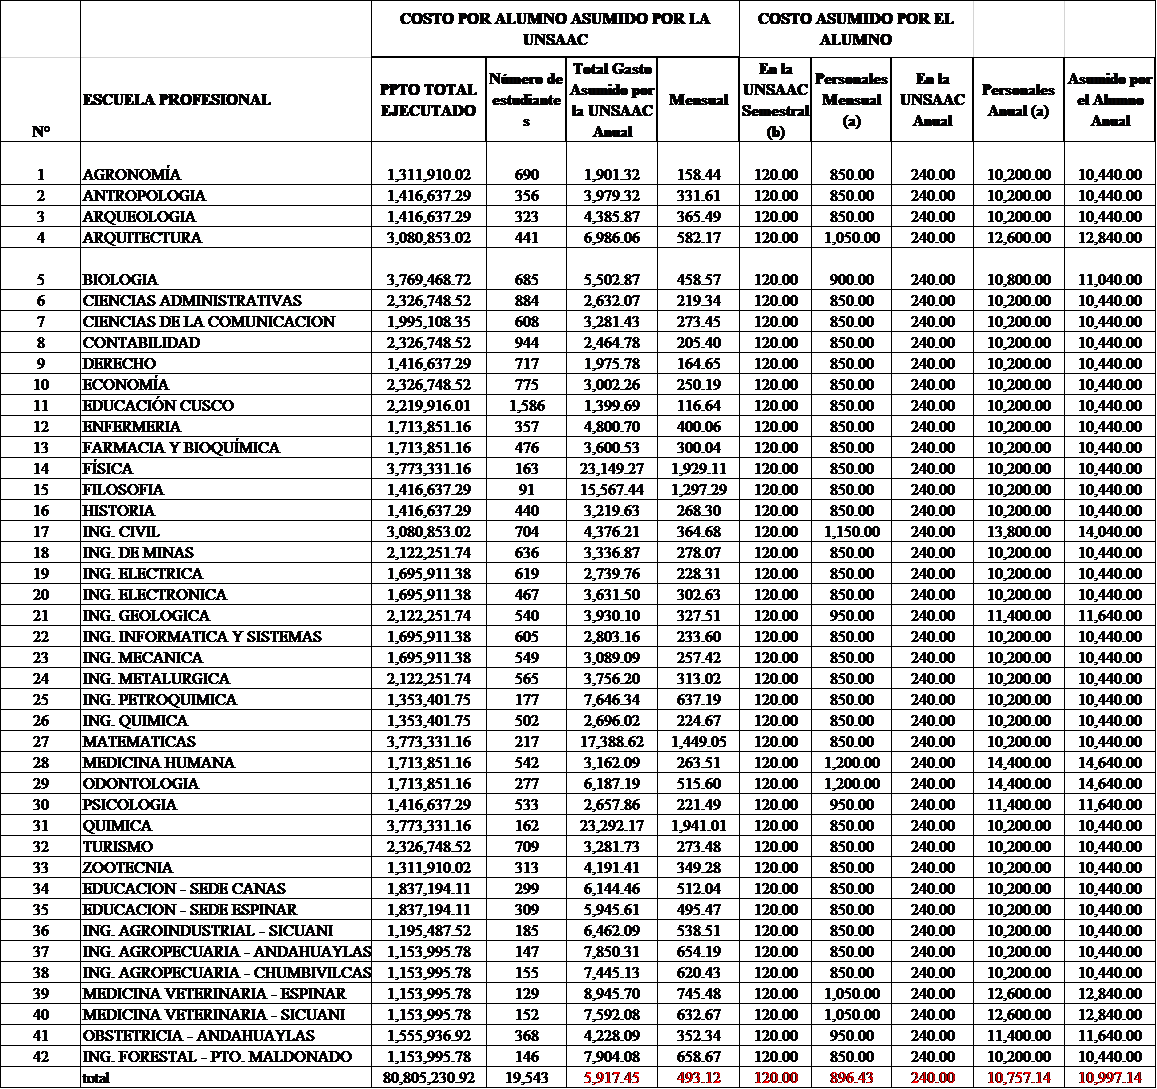
\includegraphics[keepaspectratio]{imagen/2019.png}}

}

\end{figure}%%
\begin{figure}[H]

\caption{Costo por alumno, 2020}

{\centering \pandocbounded{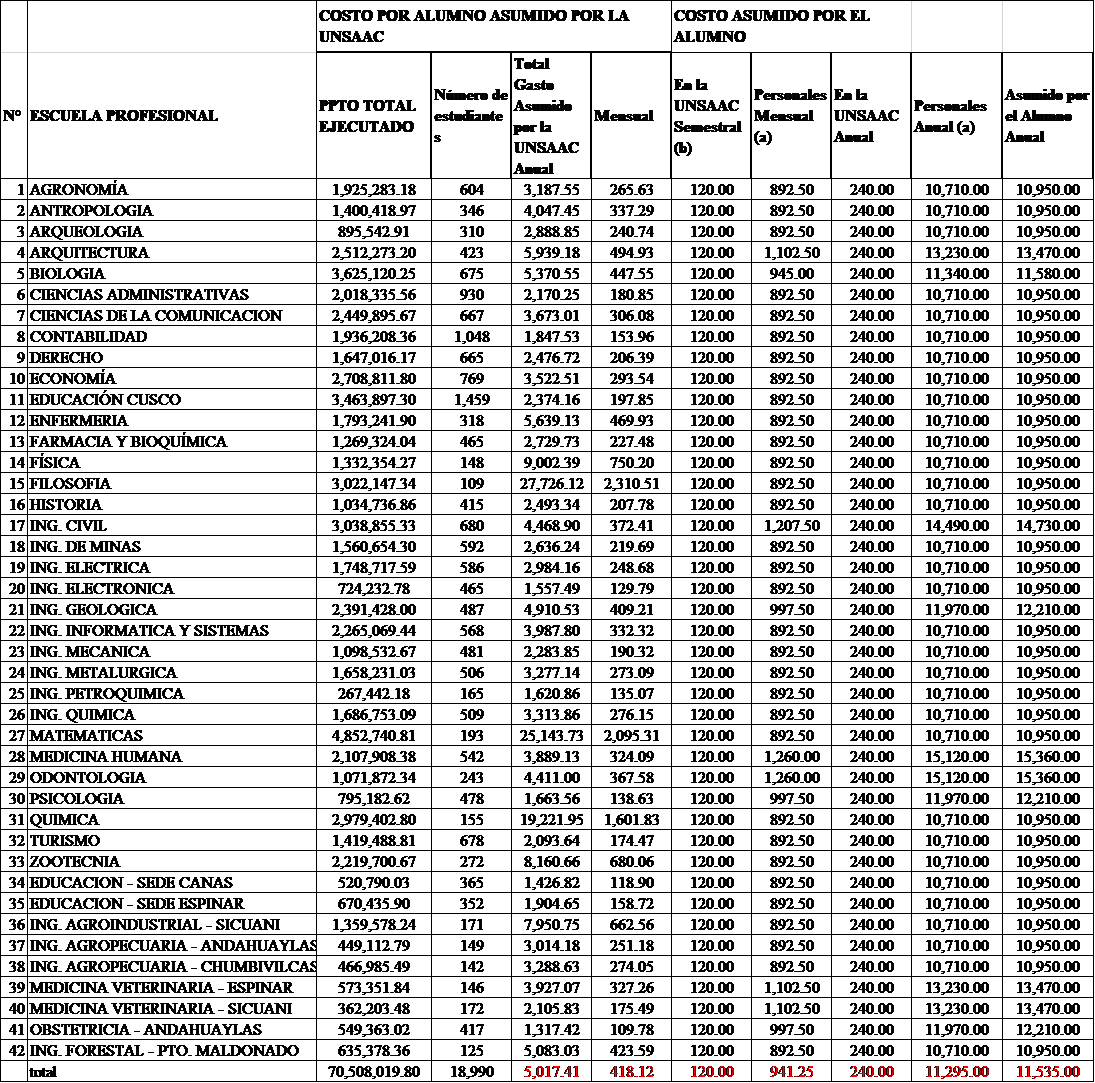
\includegraphics[keepaspectratio]{imagen/2020.png}}

}

\end{figure}%%
\begin{figure}[H]

\caption{Costo por alumno, 2021}

{\centering \pandocbounded{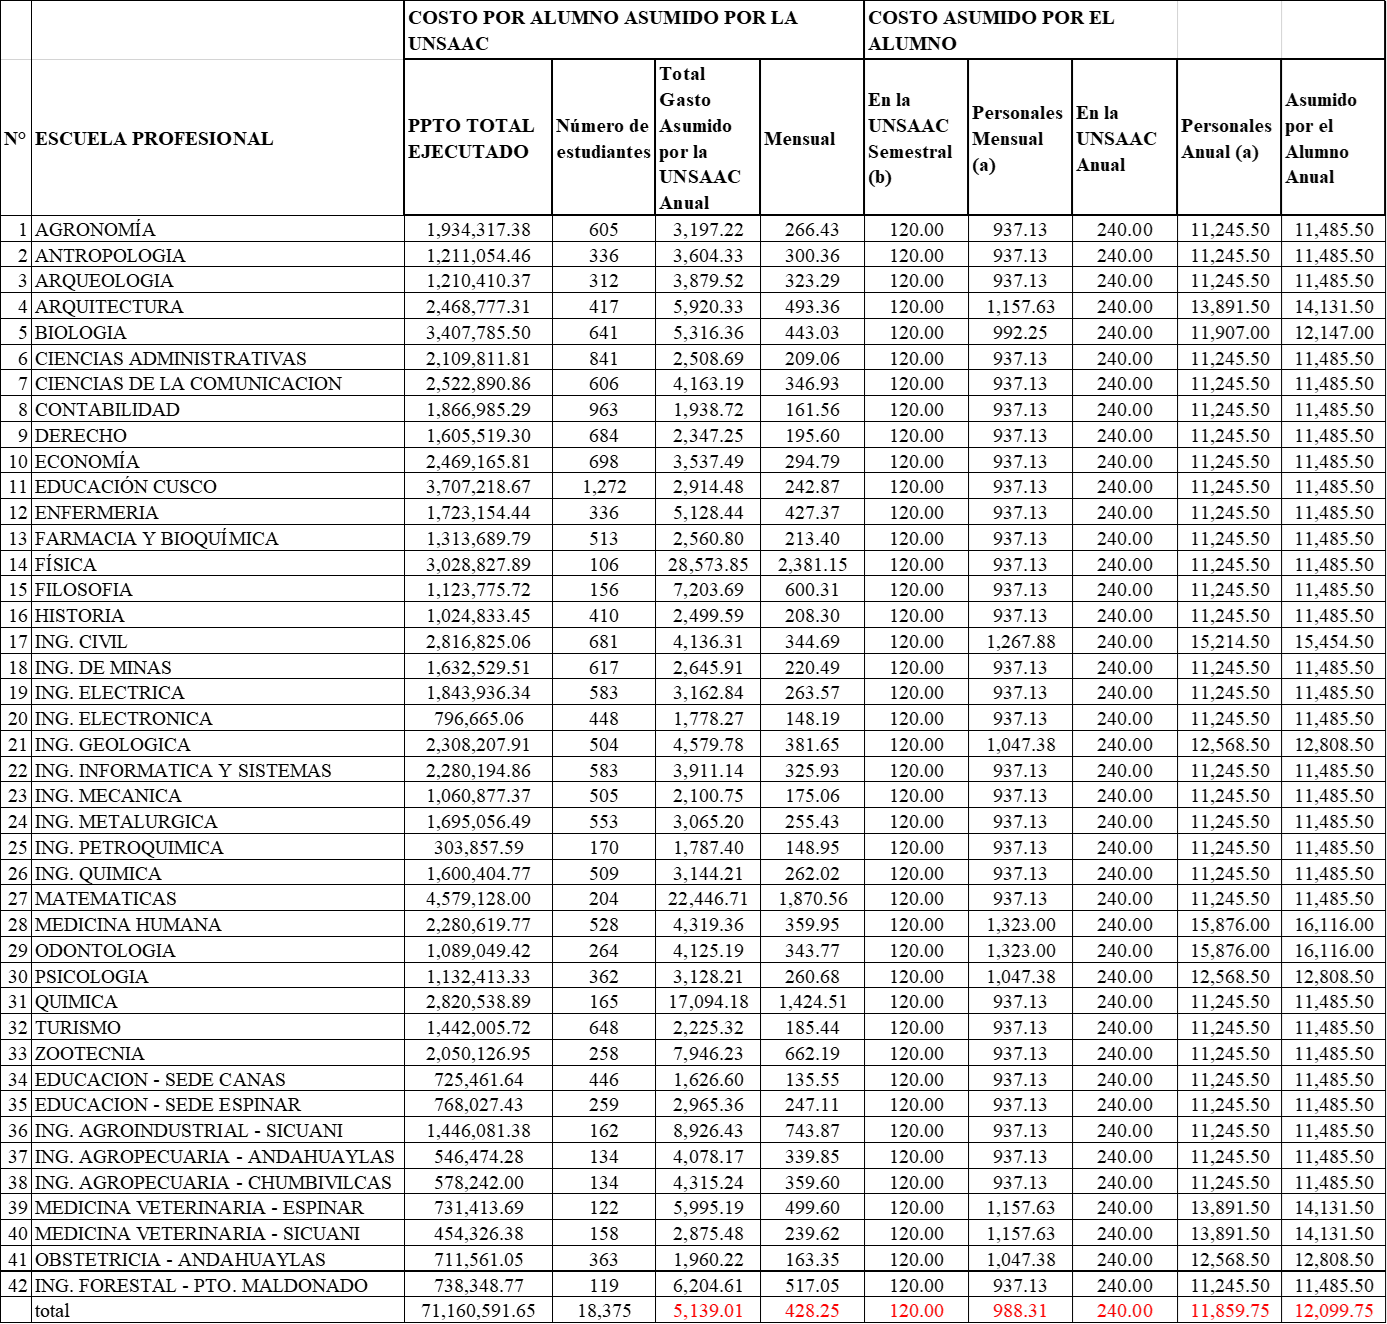
\includegraphics[keepaspectratio]{imagen/2021.png}}

}

\end{figure}%%
\begin{figure}[H]

\caption{Costo por alumno, 2022}

{\centering \pandocbounded{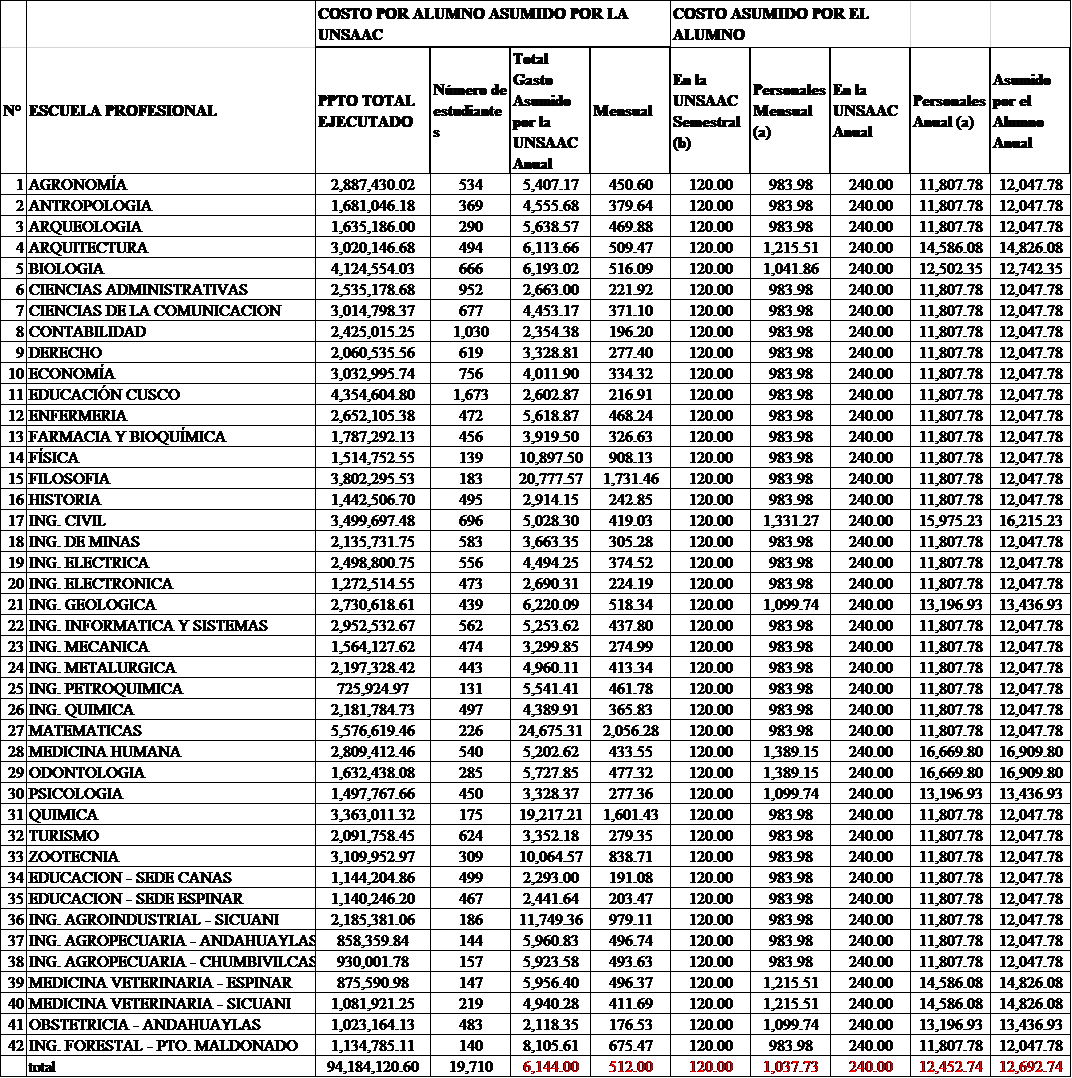
\includegraphics[keepaspectratio]{imagen/2022.png}}

}

\end{figure}%%
\begin{figure}[H]

\caption{Costo por alumno, 2023}

{\centering \pandocbounded{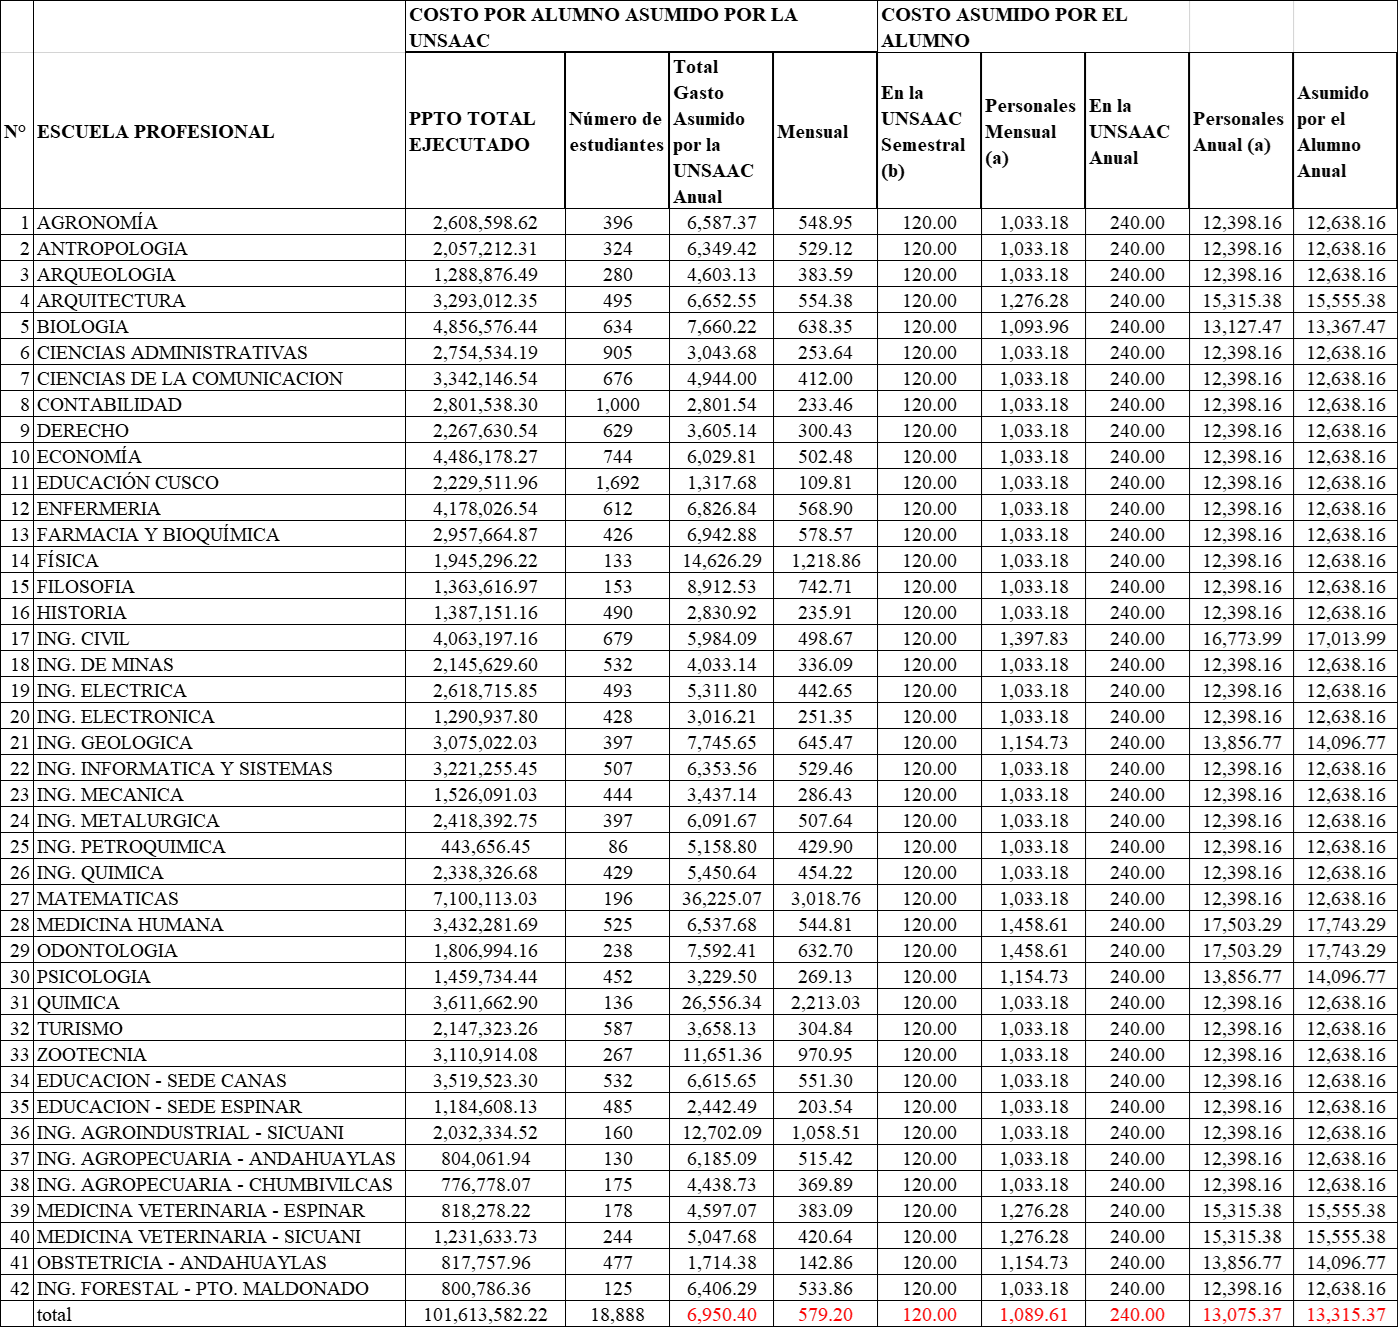
\includegraphics[keepaspectratio]{imagen/2023.png}}

}

\end{figure}%

\pagebreak

\section{Diciembre}\label{diciembre}

\subsection{Elaboracion de estadísticos de presupuesto 2019-2023
(correcciones)}\label{elaboracion-de-estaduxedsticos-de-presupuesto-2019-2023-correcciones}

Se realizo una revisión detallada de los estadisticos obtenidos y
estimados para cada categoria, puediendo levantarse errores en la
redacción y culminarse con la producción del documento ``EJECUCIÓN
PRESUPUESTAL DE GASTO 2019 - 2023''

\subsection{Elaboración de estadísticos de la E.P. de Ciencias de la
Comunicación}\label{elaboraciuxf3n-de-estaduxedsticos-de-la-e.p.-de-ciencias-de-la-comunicaciuxf3n}

Se recibió una solicitud de parte de la Dirección de la E.P. de Ciencias
de la Comunicación, en los que se pedía todos los estadísticos
correspondientes a dicha escuela profesional, reaizandose
satisfactoriamente dichos estadísticos, a continuación se presentan
algunos de los estadísticos presentados:

\begin{figure}[H]

\caption{Tabla de Presupuesto Total entre Recursos Ordinarios Y Recursos
Directamente Recaudados 2019 - Servicios Adecuados de Apoyo al
Estudiante (Bienestar y Asistencia Social)}

{\centering \pandocbounded{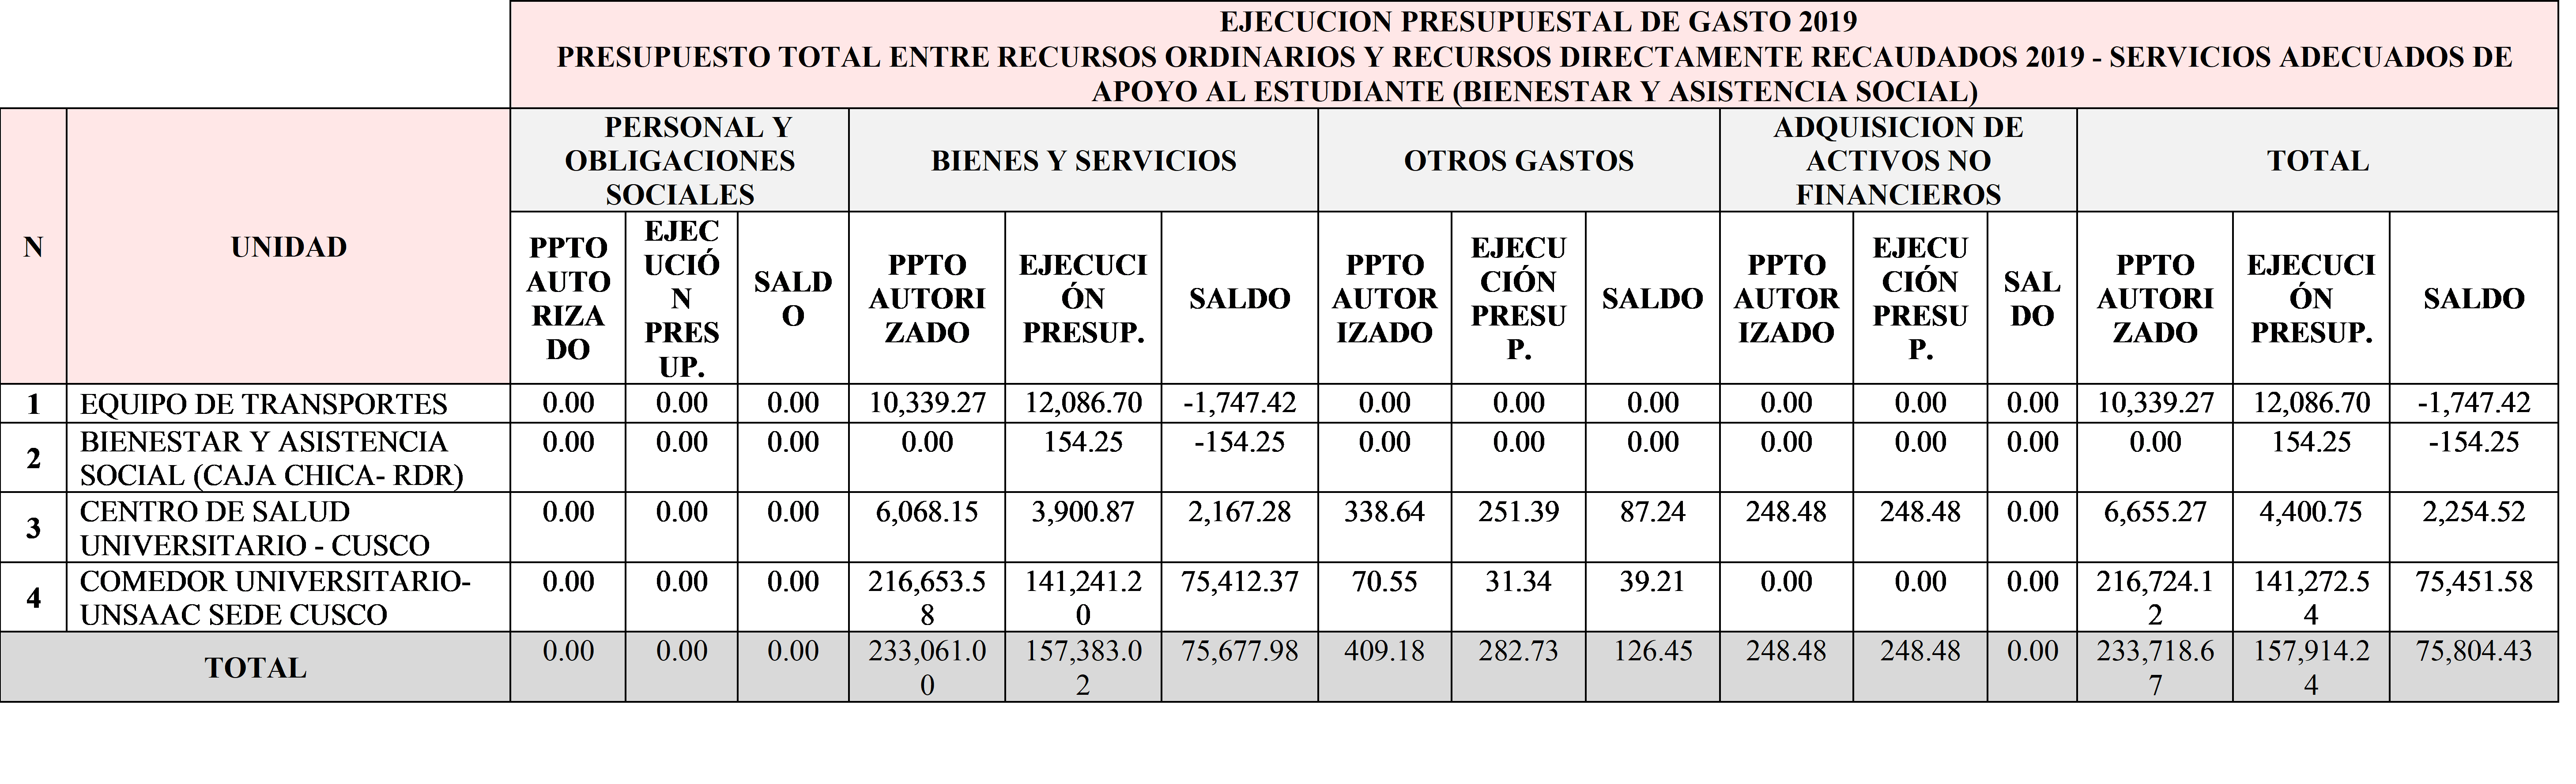
\includegraphics[keepaspectratio]{imagen/fin.png}}

}

\end{figure}%%
\begin{figure}[H]

\caption{Presupuesto Total ejecutado - E.P. Ciencias de la Comunicación
2019-2023}

{\centering \pandocbounded{
\includegraphics[keepaspectratio]{imagen/fin1.png}}

}

\end{figure}%%
\begin{figure}[H]

\caption{Costo por alumno - E.P. Ciencias de la Comunicación 2019}

{\centering \pandocbounded{
\includegraphics[keepaspectratio]{imagen/2019m.png}}

}

\end{figure}%%
\begin{figure}[H]

\caption{Costo por alumno - E.P. Ciencias de la Comunicación 2020}

{\centering \pandocbounded{
\includegraphics[keepaspectratio]{imagen/2020m.png}}

}

\end{figure}%%
\begin{figure}[H]

\caption{Costo por alumno - E.P. Ciencias de la Comunicación 2021}

{\centering \pandocbounded{
\includegraphics[keepaspectratio]{imagen/2021m.png}}

}

\end{figure}%%
\begin{figure}[H]

\caption{Costo por alumno - E.P. Ciencias de la Comunicación 2022}

{\centering \pandocbounded{
\includegraphics[keepaspectratio]{imagen/2022m.png}}

}

\end{figure}%%
\begin{figure}[H]

\caption{Costo por alumno - E.P. Ciencias de la Comunicación 2023}

{\centering \pandocbounded{
\includegraphics[keepaspectratio]{imagen/2023m.png}}

}

\end{figure}%

\subsection{Elaboración de proyecciones estadísticas
2024-2034}\label{elaboraciuxf3n-de-proyecciones-estaduxedsticas-2024-2034}

Se tiene que la Unidad de Estadística presenta regularmente una
publicación acerca de las proyecciones estadísticas, las que
correspondian a la publicación eran proyecciones estadística del
2024-2034, se realizaron proyecciones con respecto a las siguientes
variables universitarias:

\begin{itemize}
\tightlist
\item
  Vacantes
\item
  Postulantes
\item
  Ingresantes
\item
  Matriculados
\item
  Egresados
\item
  Graduados
\item
  Titulados
\item
  Docentes nombrados
\item
  Docentes contratados
\item
  Personal administrativo nombrado y contratado
\end{itemize}

Teniendose las siguientes proyecciones:

\begin{figure}[H]

\caption{Proyección de vacantes 2024-2034}

{\centering \pandocbounded{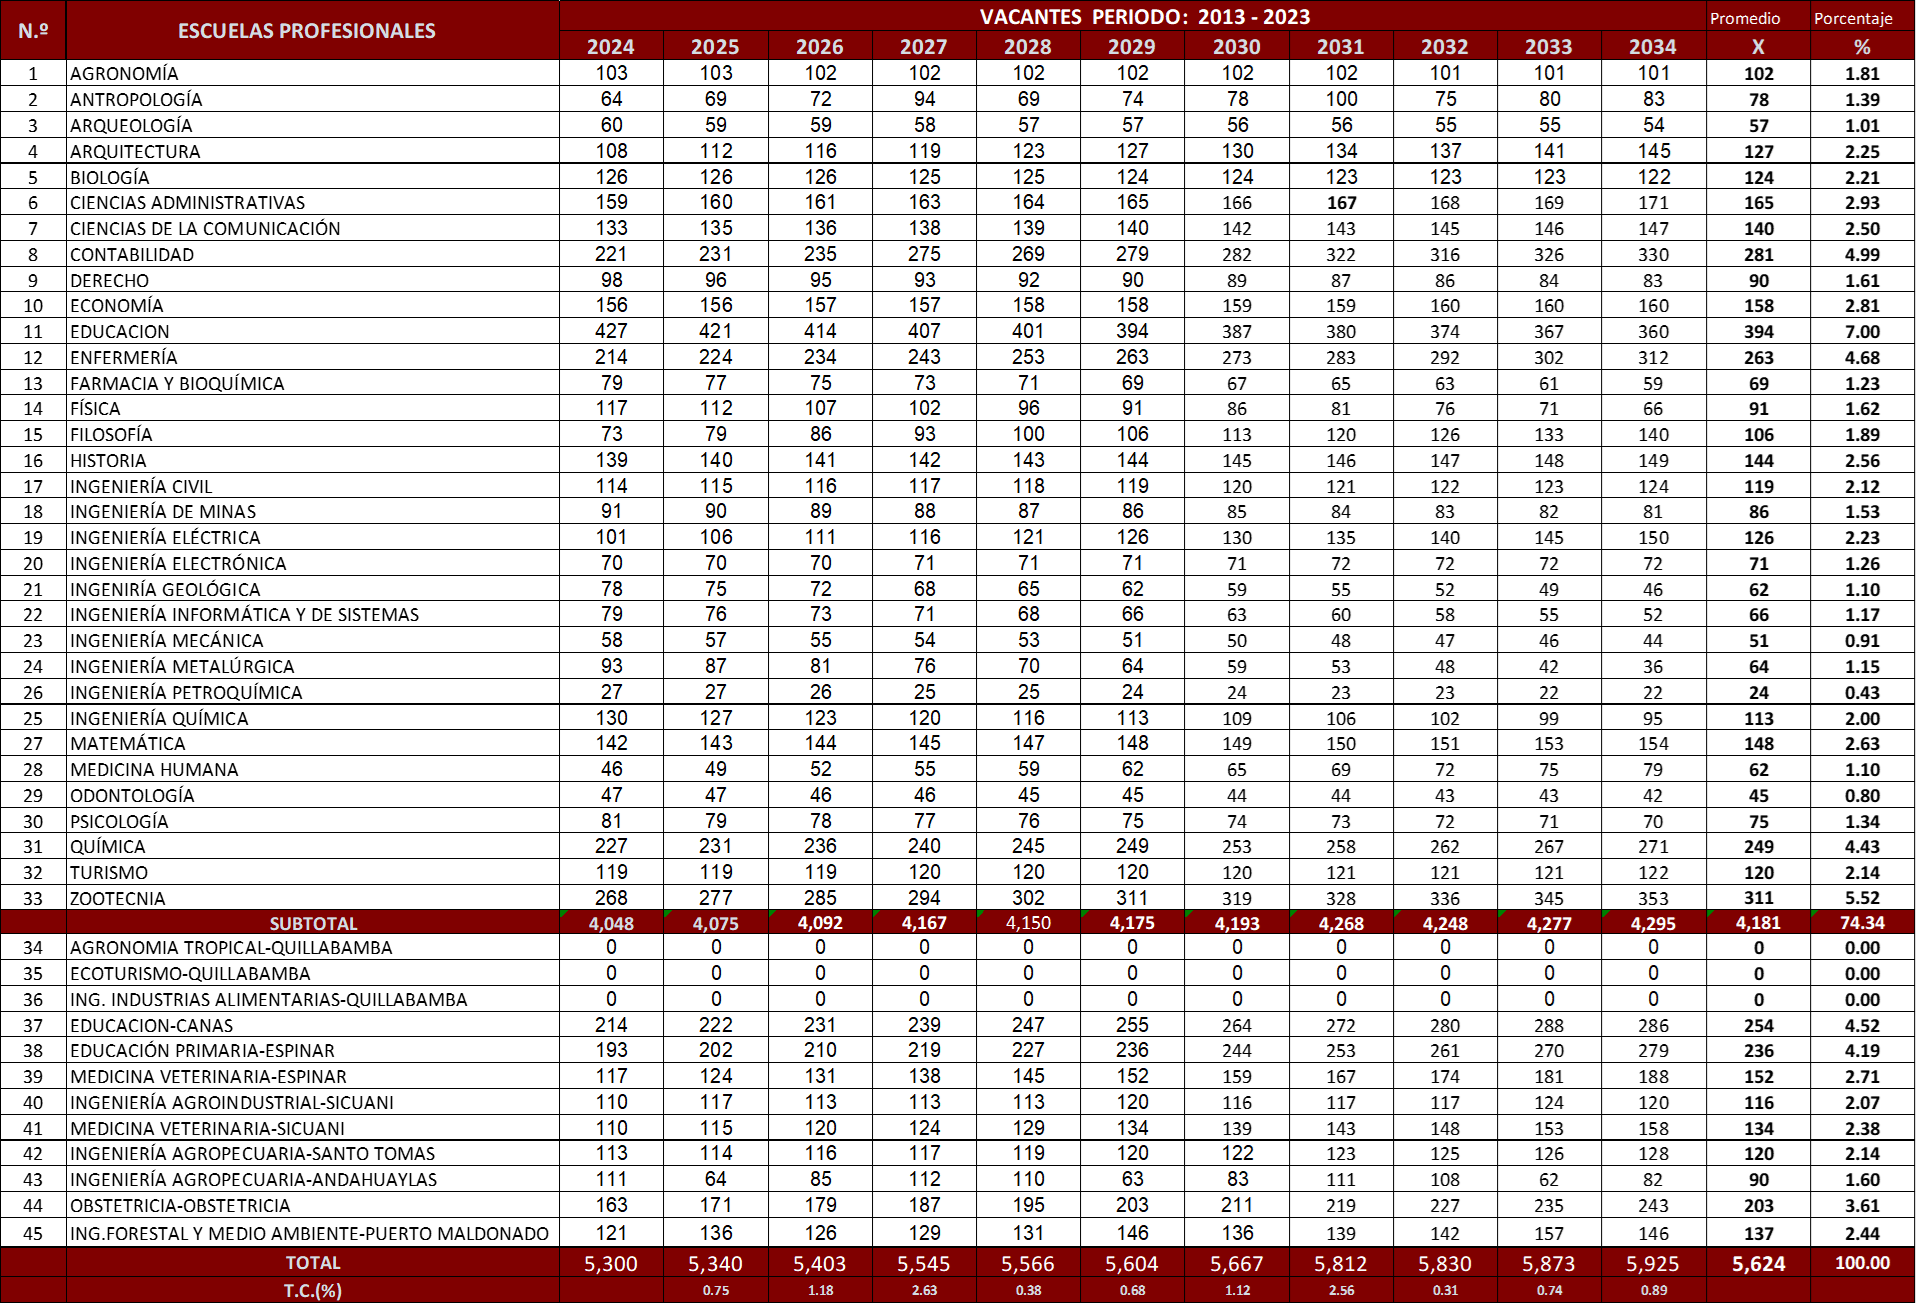
\includegraphics[keepaspectratio]{imagen/vac.png}}

}

\end{figure}%%
\begin{figure}[H]

\caption{Proyección de postulantes 2024-2034}

{\centering \pandocbounded{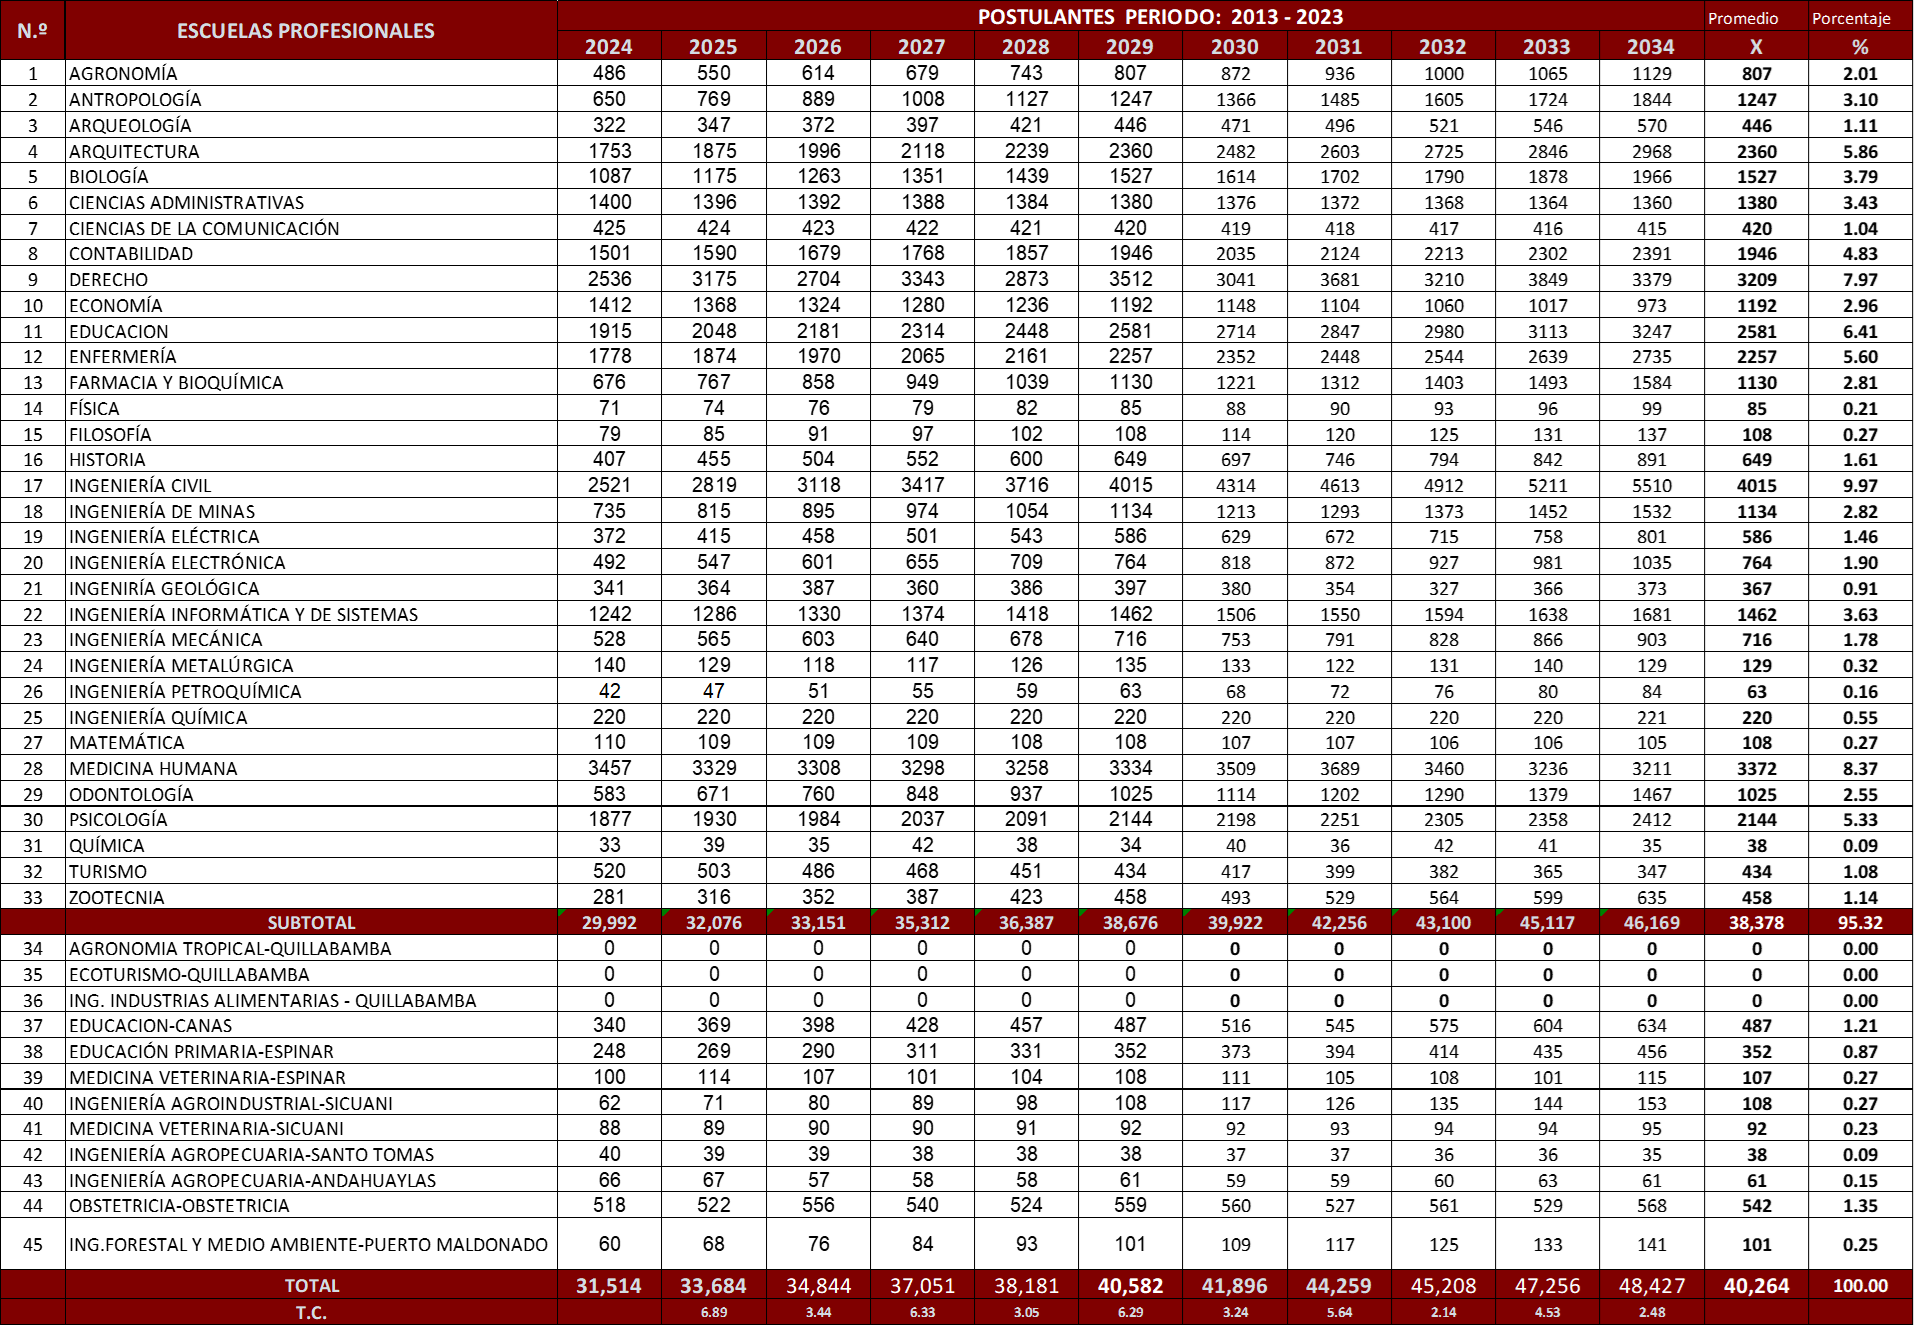
\includegraphics[keepaspectratio]{imagen/pos.png}}

}

\end{figure}%%
\begin{figure}[H]

\caption{Proyección de ingresantes 2024-2034}

{\centering \pandocbounded{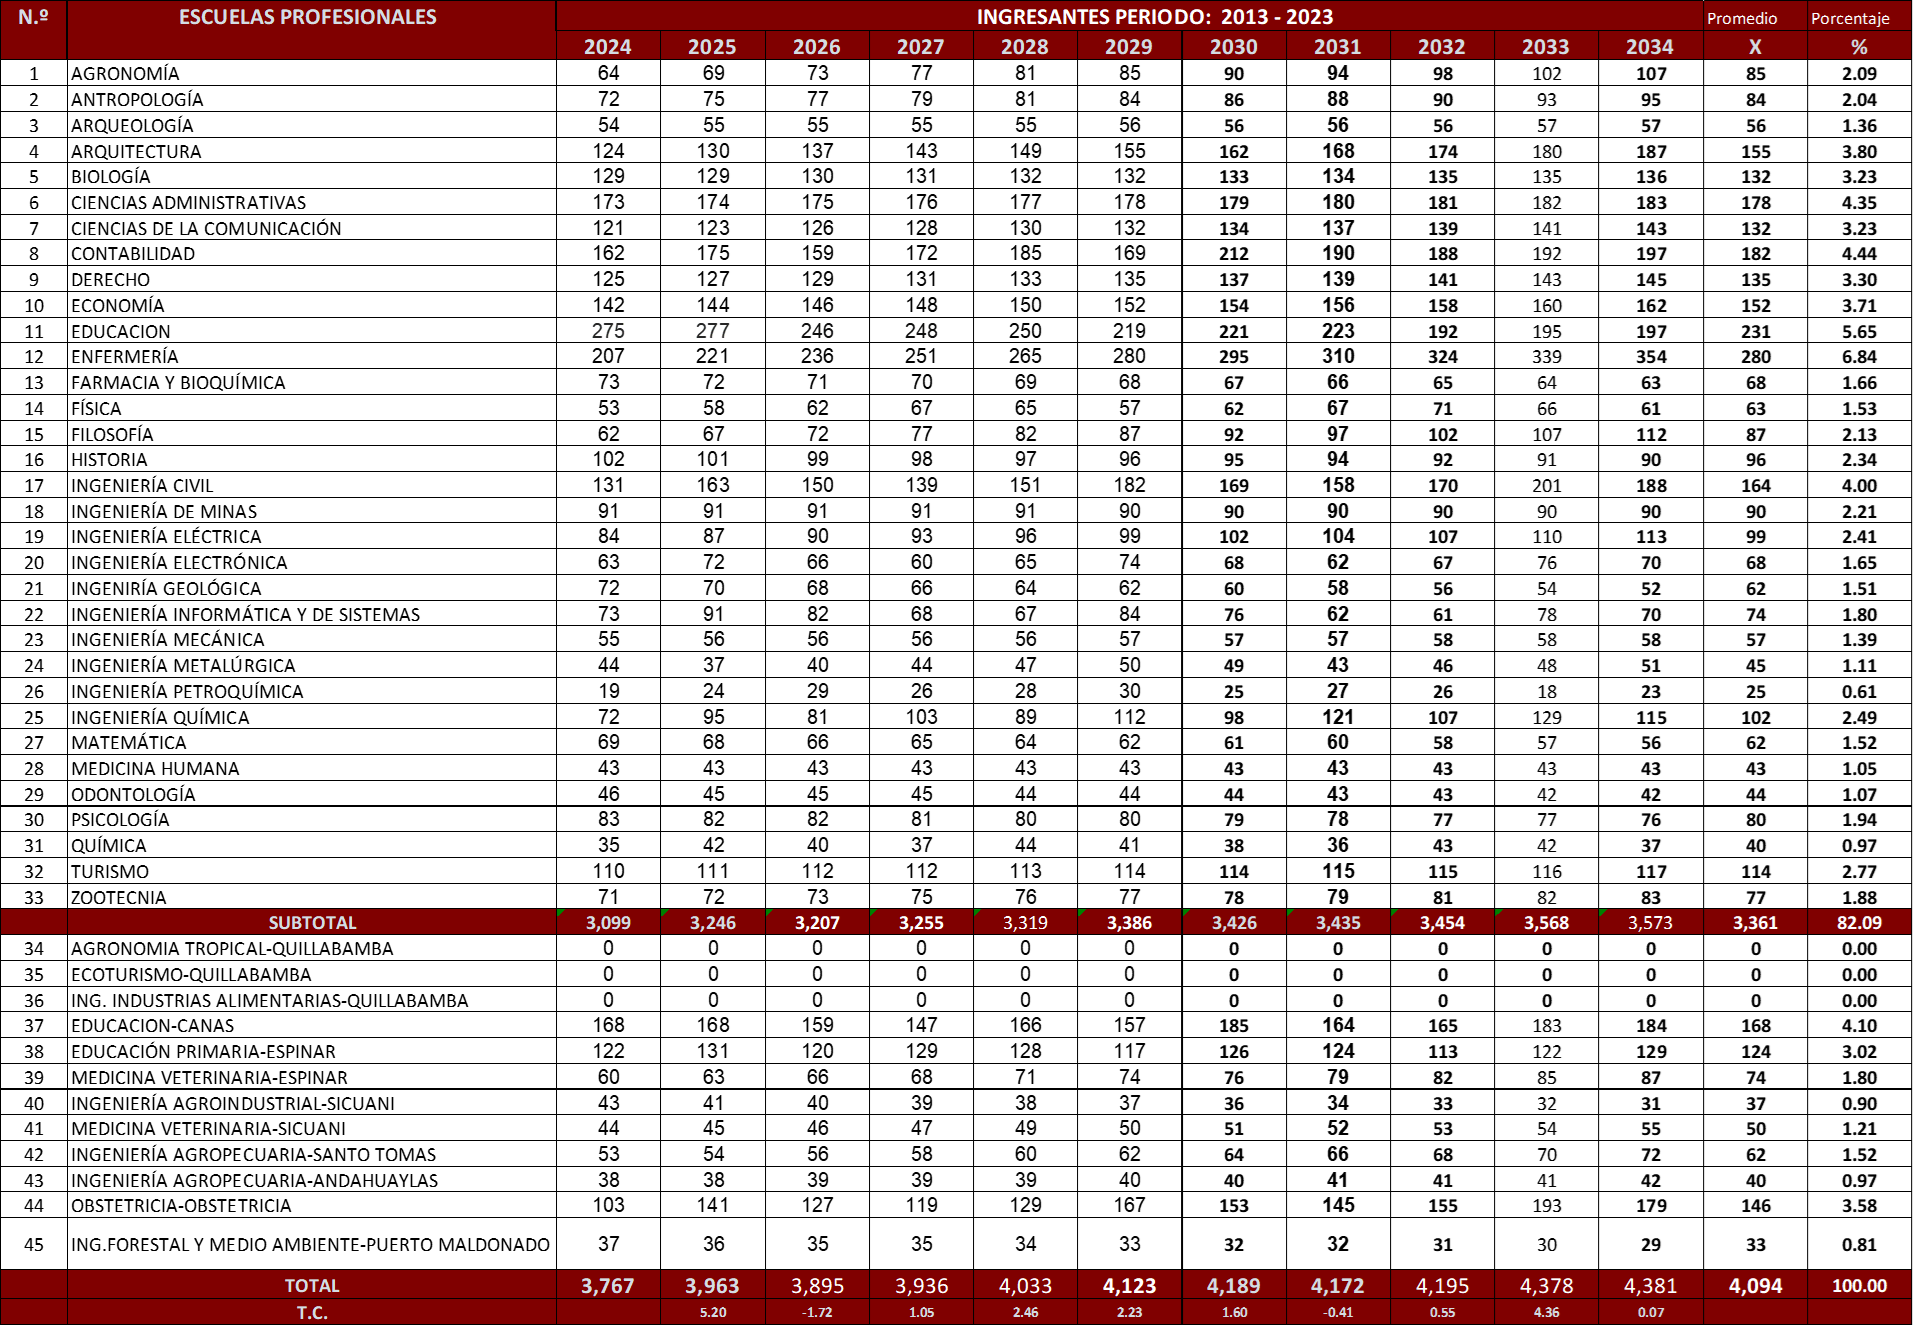
\includegraphics[keepaspectratio]{imagen/ing.png}}

}

\end{figure}%%
\begin{figure}[H]

\caption{Proyección de matriculados 2024-2034}

{\centering \pandocbounded{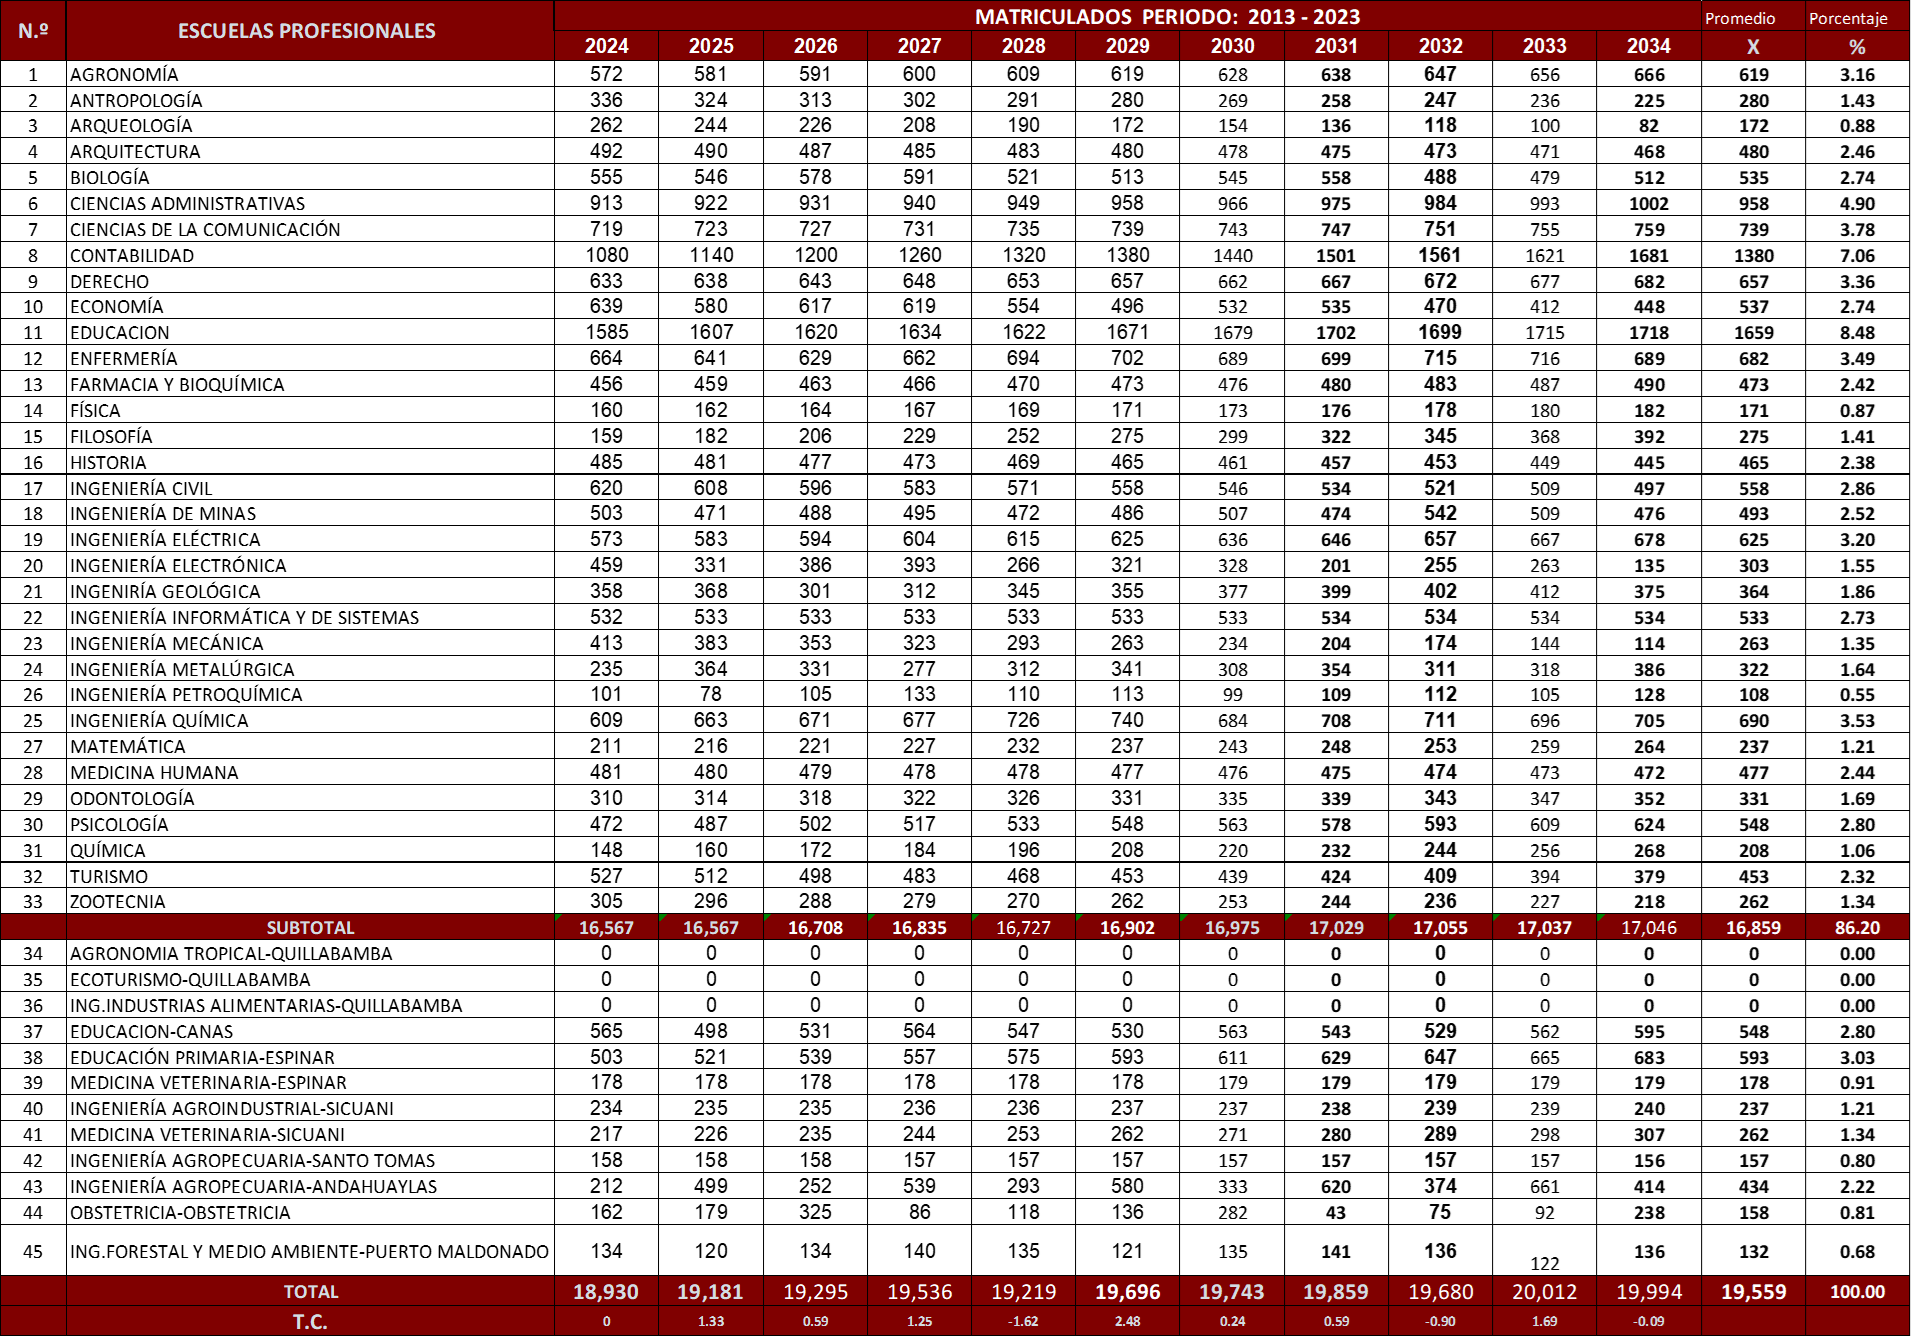
\includegraphics[keepaspectratio]{imagen/mat.png}}

}

\end{figure}%%
\begin{figure}[H]

\caption{Proyección de egresados 2024-2034}

{\centering \pandocbounded{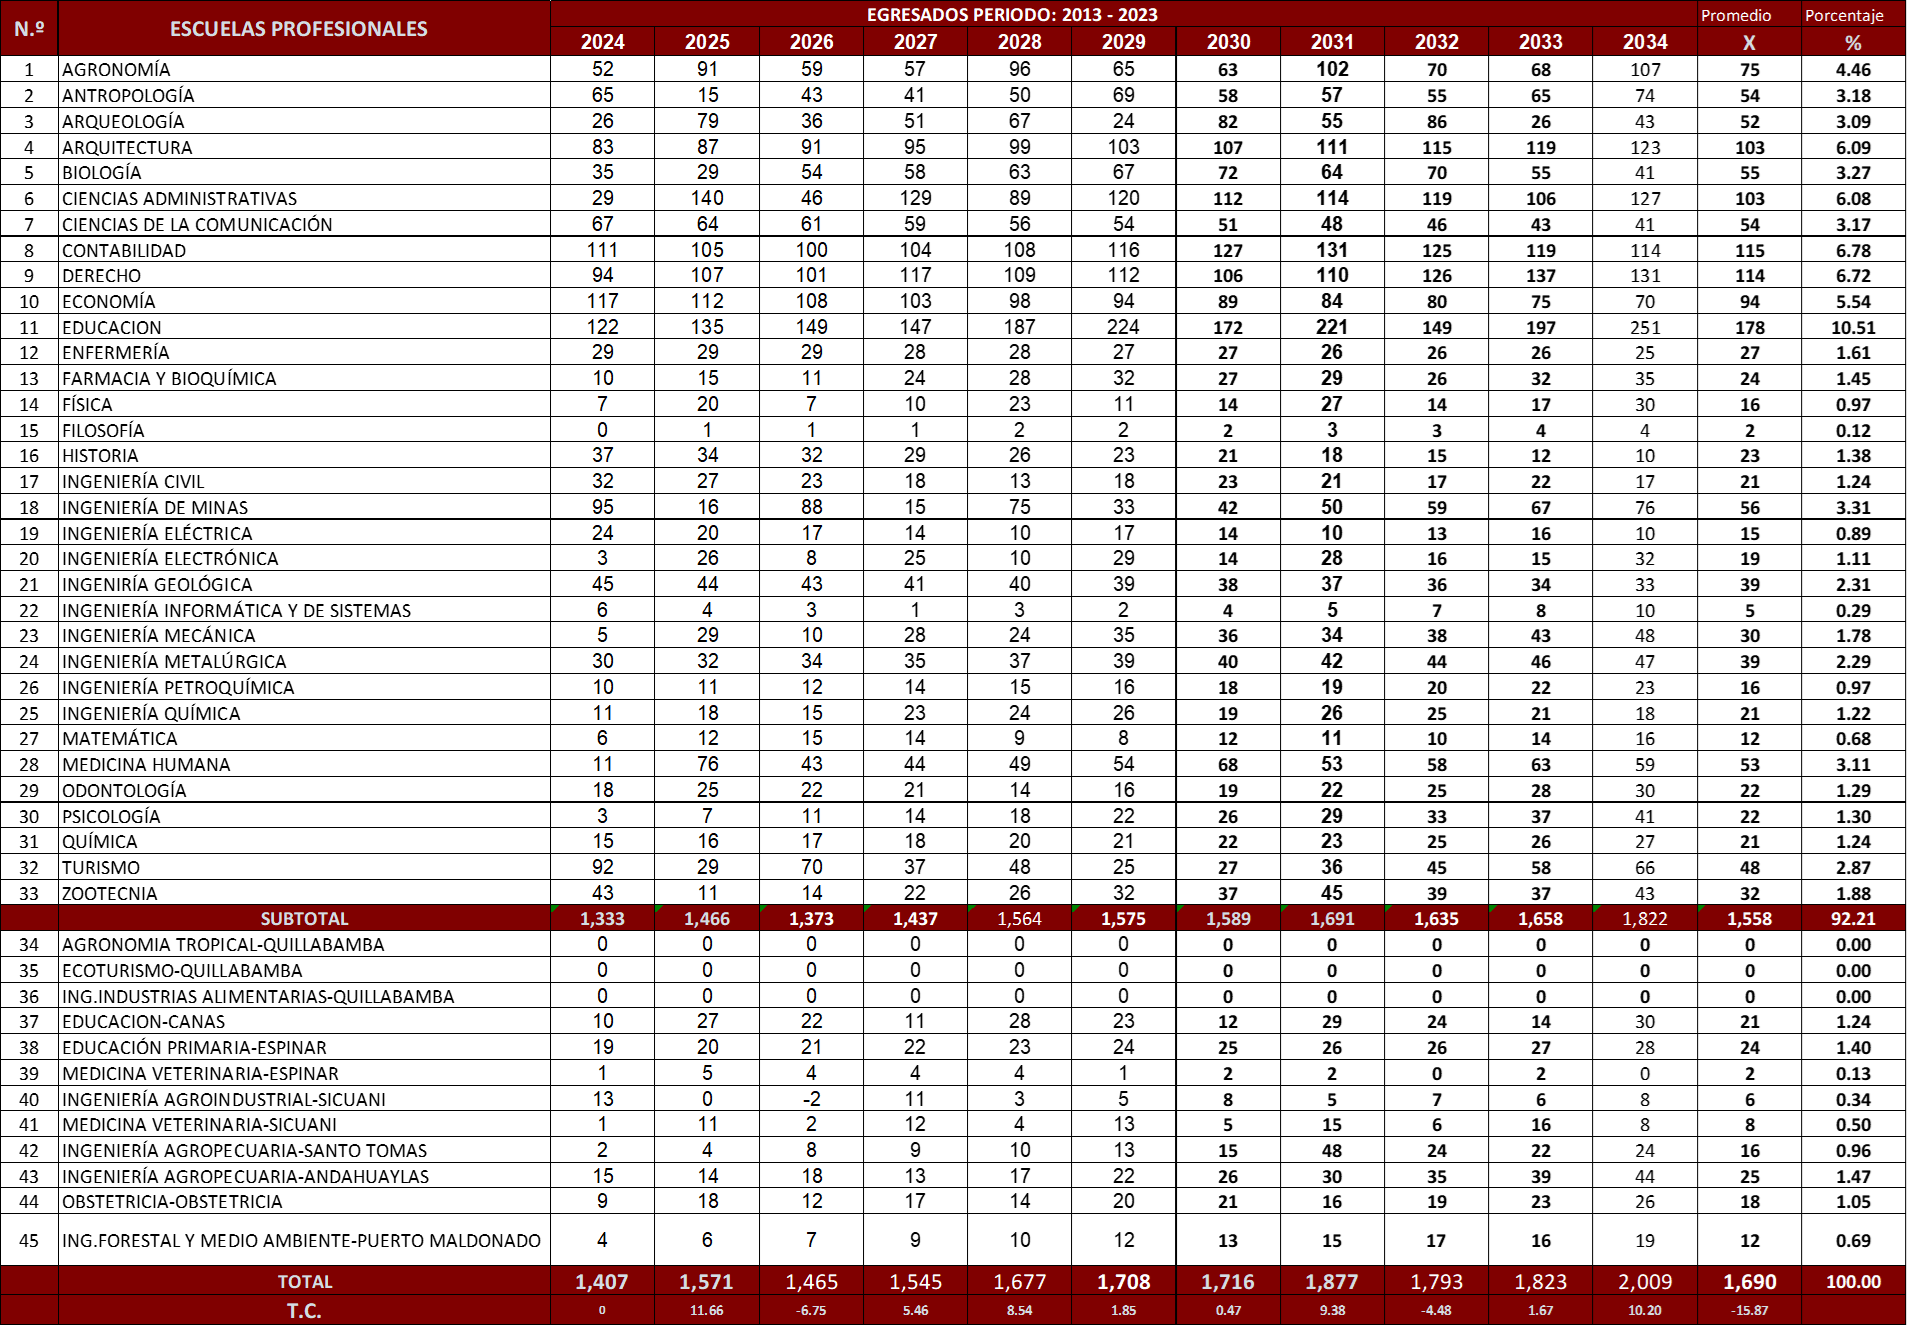
\includegraphics[keepaspectratio]{imagen/egr.png}}

}

\end{figure}%%
\begin{figure}[H]

\caption{Proyección de graduados 2024-2034}

{\centering \pandocbounded{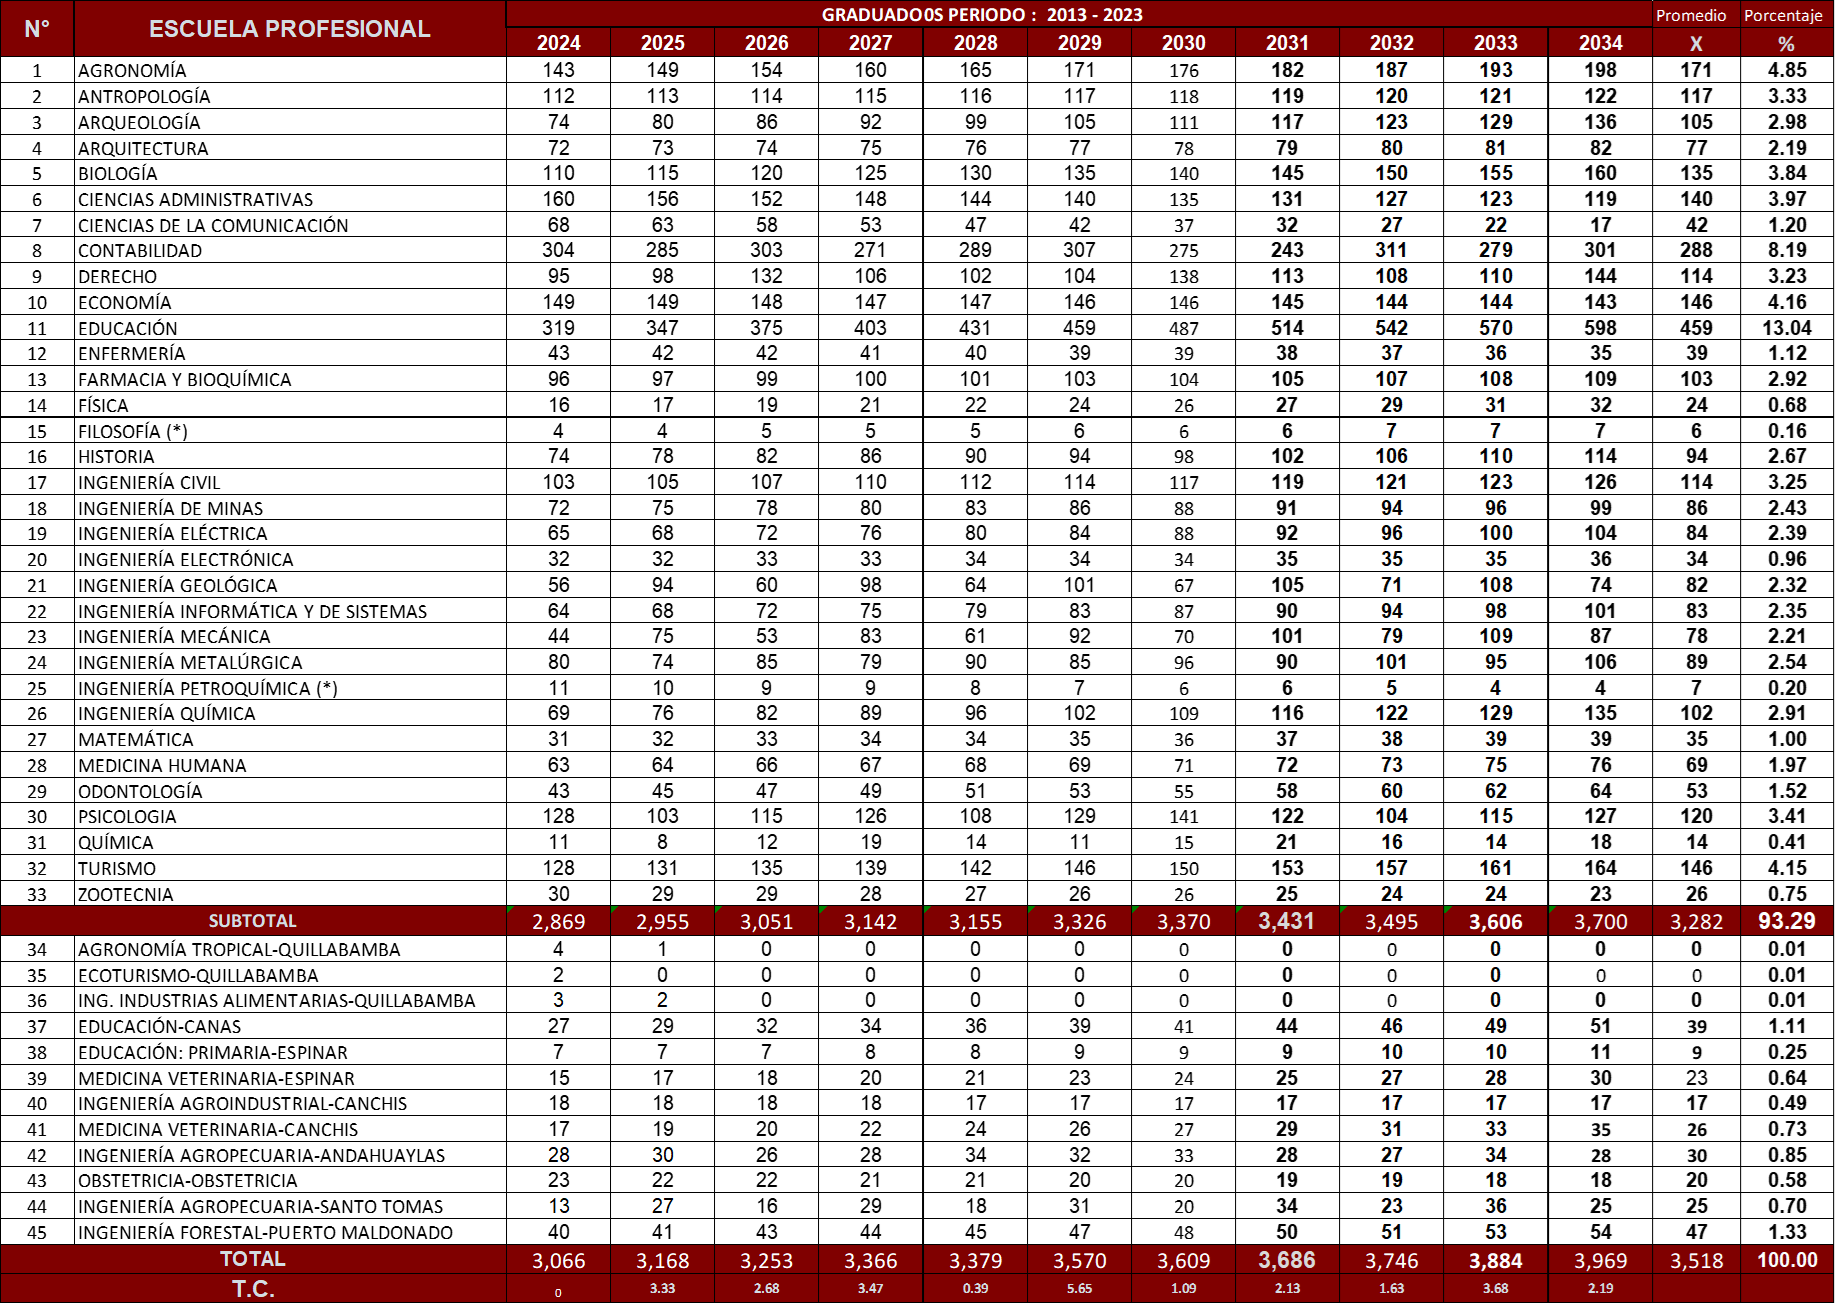
\includegraphics[keepaspectratio]{imagen/gra.png}}

}

\end{figure}%%
\begin{figure}[H]

\caption{Proyección de titulados 2024-2034}

{\centering \pandocbounded{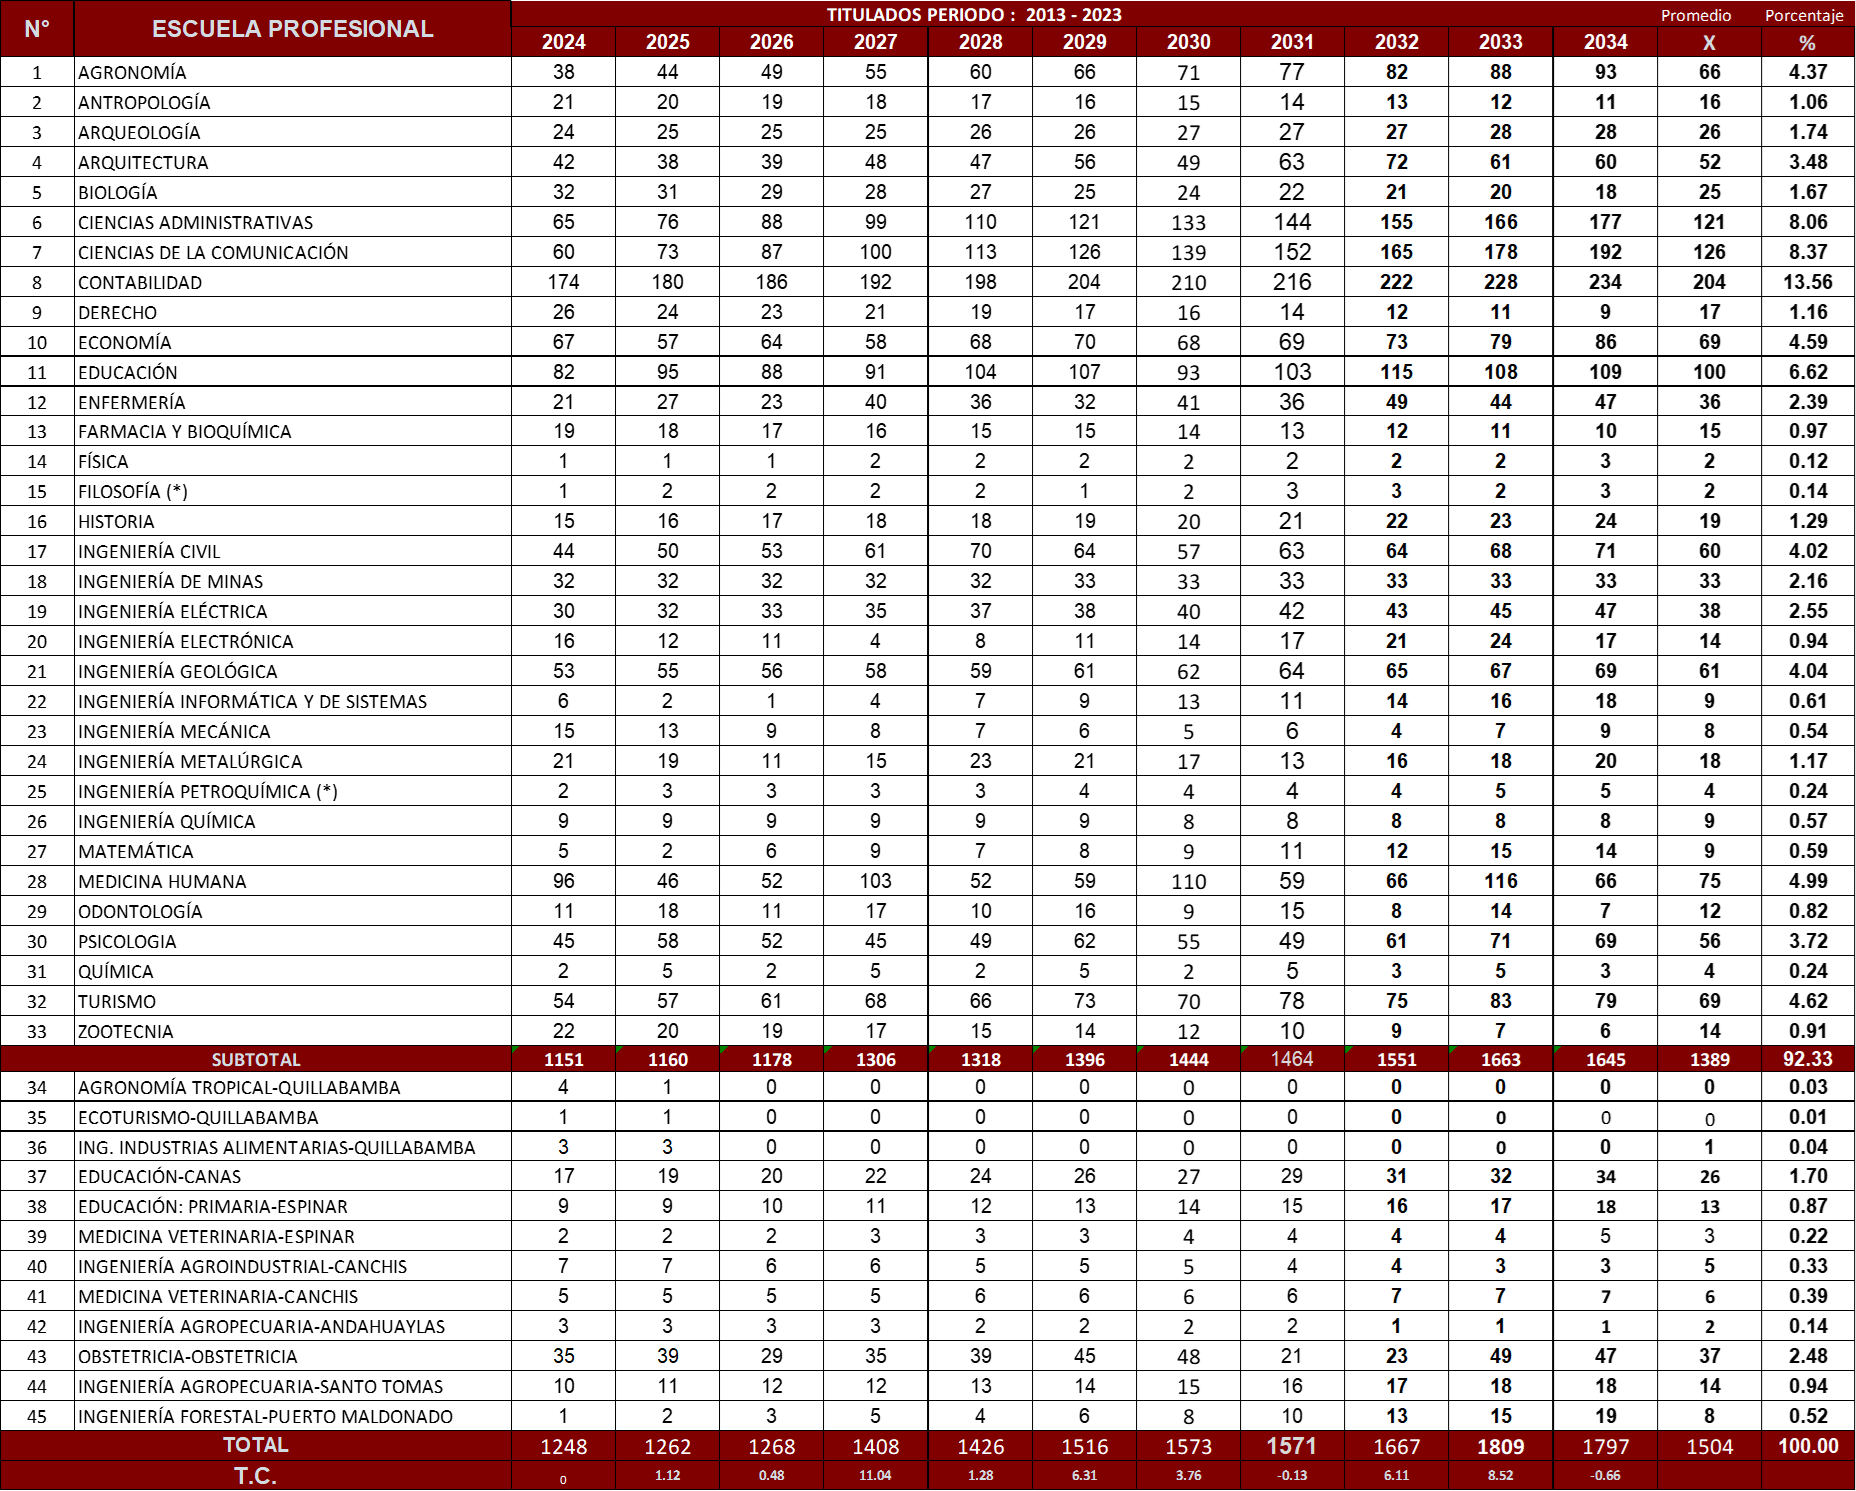
\includegraphics[keepaspectratio]{imagen/tit.png}}

}

\end{figure}%%
\begin{figure}[H]

\caption{Proyección de docentes nombrados 2024-2034}

{\centering \pandocbounded{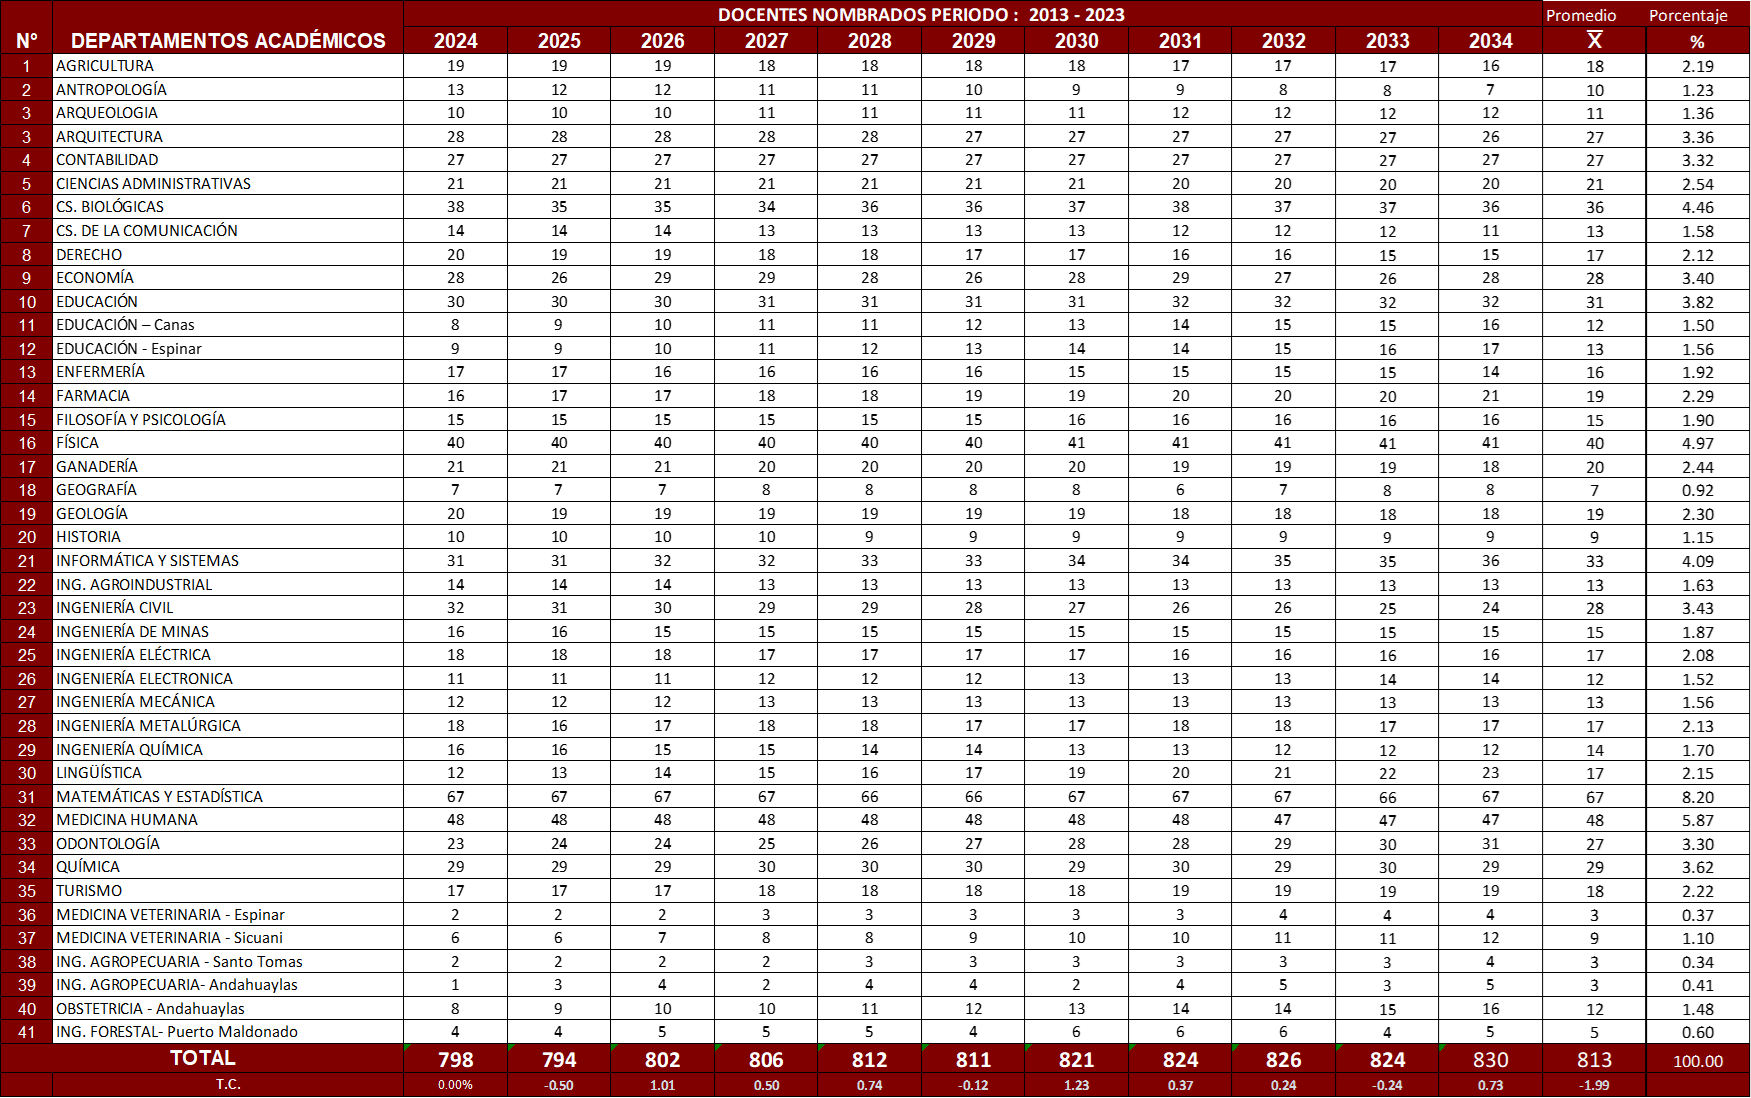
\includegraphics[keepaspectratio]{imagen/dnom.png}}

}

\end{figure}%%
\begin{figure}[H]

\caption{Proyección de docentes contratados 2024-2034}

{\centering \pandocbounded{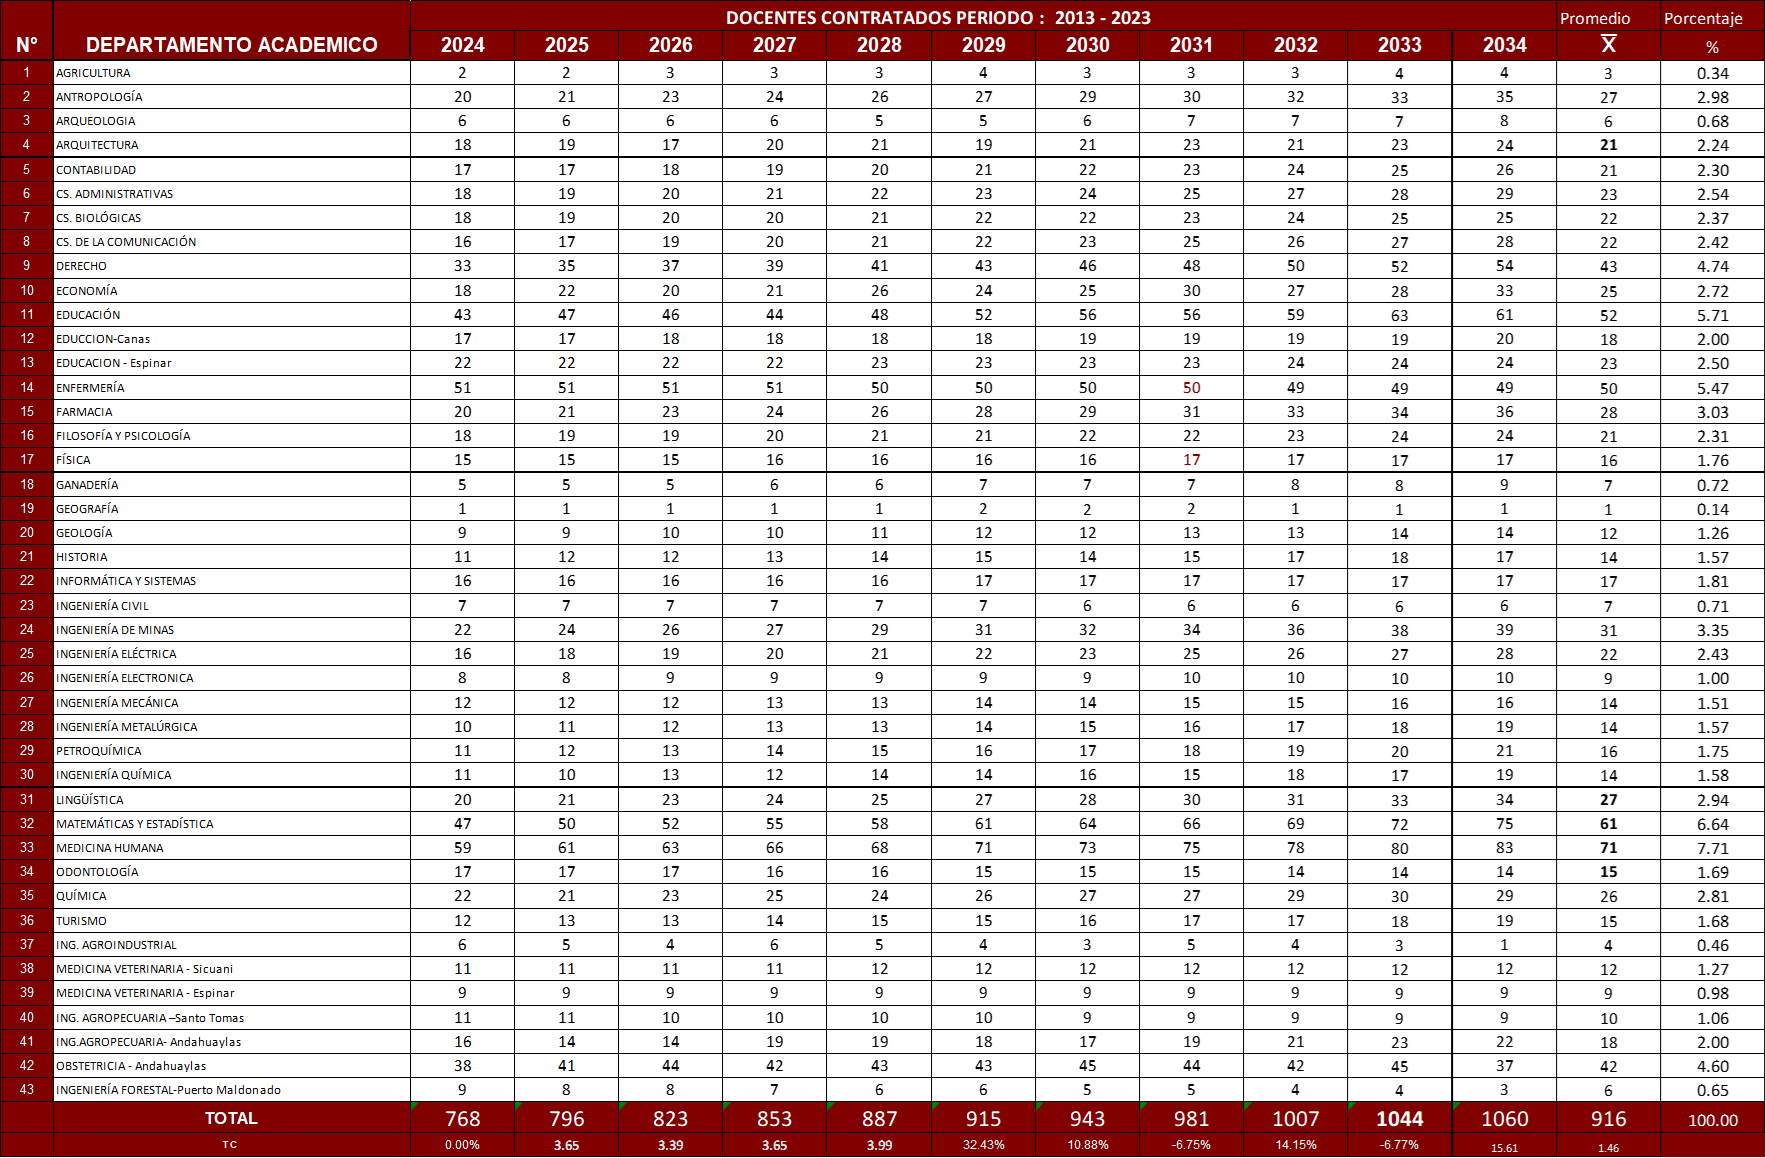
\includegraphics[keepaspectratio]{imagen/dcon.png}}

}

\end{figure}%%
\begin{figure}[H]

\caption{Proyección de personal administrativo nombrado y contratado
2024-2034}

{\centering \pandocbounded{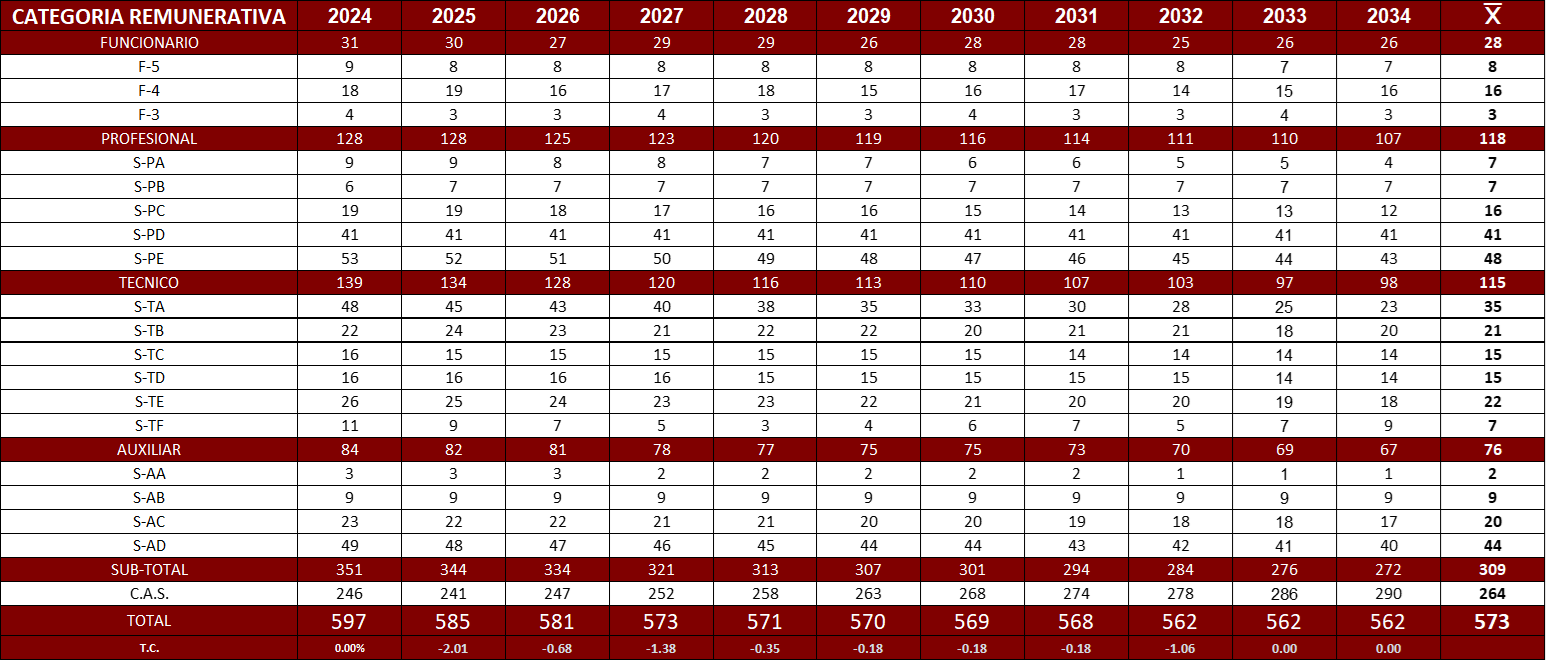
\includegraphics[keepaspectratio]{imagen/per.png}}

}

\end{figure}%

\bookmarksetup{startatroot}

\chapter{Conclusiones}\label{conclusiones}

La realización de Prácticas pre-Profesionales en la Unidad de
Estadística, me permitió obtener una visión más profunda desde el
enfoque estadístico sobre la situación de la Universidad Nacional de San
Antonio abad del Cusco, aplicandose la estadística descriptiva en los
datos que se van proporcionando.

Este entorno hace que uno se evalue y considere soluciones fuera del
contexto habitual, se tuvo la oportunidad de aplicar los conocimientos
de estadistica descriptiva y el office, conocimientos y habilidades
adquiridas durante la formación académica.

El analisis descriptivo es una labor sencilla pero pesada debido a la
pérdida de información que es recurrente en las bases de datos que la
Universidad le proporciona a la Unidad de Estadística.

Se aprendió bastante sobre las funciones de la Unidad de Estadística y
se resalta la posición de ser servicial dentro de la Unidad de
Estadistica para con la comunidad universitaria.

Es por ello que agradezco a la Universidad Nacional de San Antonio Abad
del Cusco por brindarme la oportunidad de realizar las Prácticas
Pre-Profesionales en la Unidad de Estadística, permitiéndome aplicar
parte de los conocimientos adquiridos en la estadística. Asimismo,
agradezco al Econ. Carlos Huamán Aguilar por permitirme la oportunidad
de realizar las prácticas.

\bookmarksetup{startatroot}

\chapter{Recomendaciones y
Sugerencias}\label{recomendaciones-y-sugerencias}

Viendo las dificultades que se tuvieron, me gustaria que el Centro de
Cómputo administre con más orden las bases de datos, es más sería genial
que la Universidad implementase una licencia de SQL para el manejo de
datos y el modelamiento correspondiente, la universidad deberia
aprovechar la tecnologia y la ciencia de datos para mejorar en los
pocesos que concierne necesarios.

Tambien me gustaria que en la Unidad de Estadística se implementase
procesos completos de la ciencia de datos, que no solo abarque la
estadística descriptiva, el compendio estadístico que se presenta cada
año, es rutinario y no despierta el interés de su elaboración para el
público en general, sería basante interesante que se pudiese aplicar el
machine learning para el modelamiento y la presentación de resultados.

Sugiero a los estudiantes que buscan realizar Prácticas
Pre-Profesionales, busquen explorar e implementar nuevas herramientas y
procesos de análisis estadístico, se tiene al R y Python como software
estadísticos que cada vez van ampliando nuevos procesos, el cual pueden
optimizar el trabajo que se realiza. La importancia de los conocimientos
en ofimática han ido perdiendo su relevancia pero para lo que se realiza
en la Unidad de Estadística es esencial tenerlo presente.

Dado esto agradezco por los conociemientos adquiridos durante la
duración de las Prácticas Pre-Profesionales (PPP) en la Unidad de
Estadística, tener una vision descriptiva de esta, hace que nuevas ideas
de mejora surgan.

\bookmarksetup{startatroot}

\chapter{Asistencia}\label{asistencia}

\pandocbounded{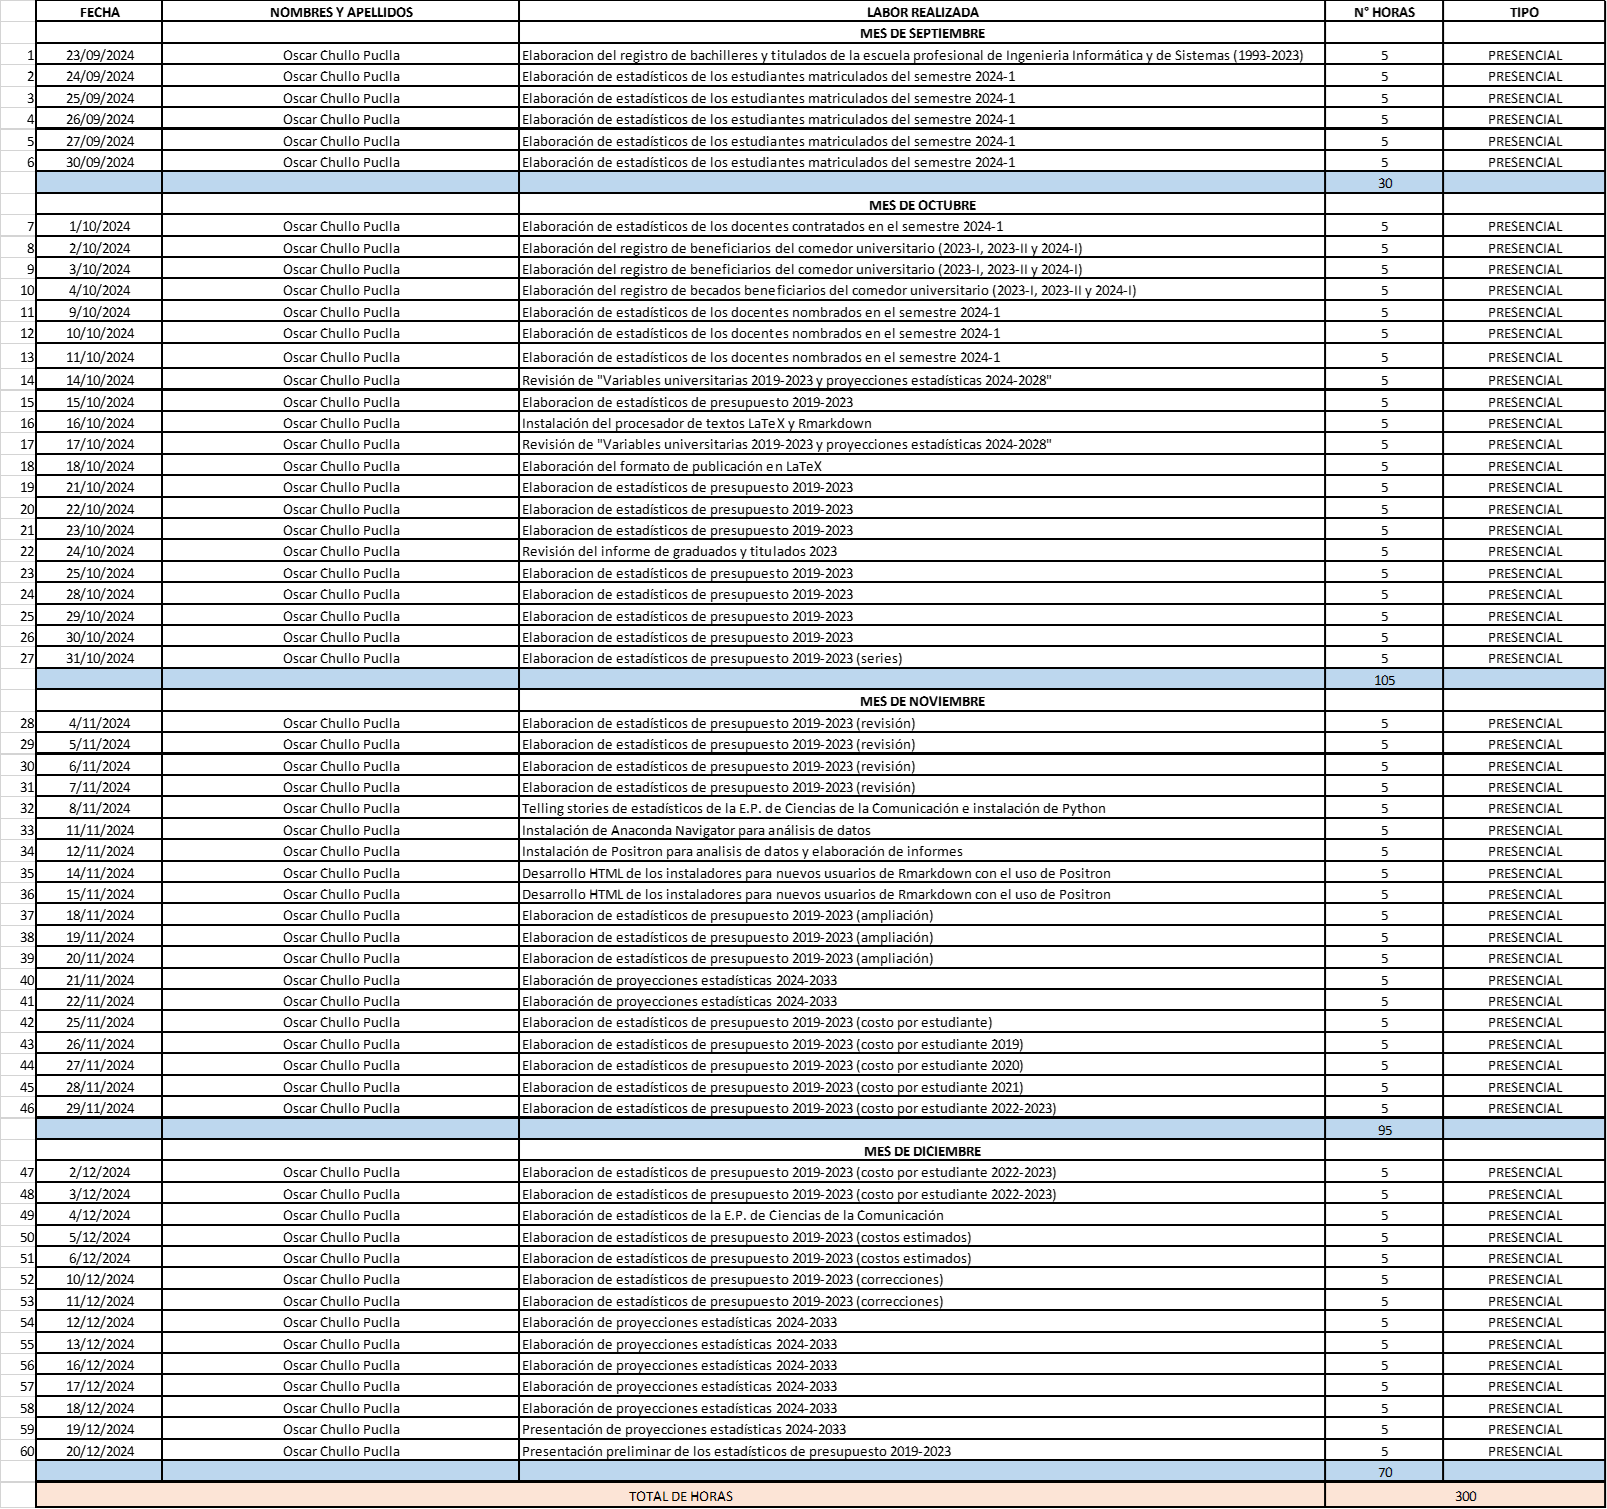
\includegraphics[keepaspectratio]{imagen/asis.png}}

\bookmarksetup{startatroot}

\chapter*{Referencias}\label{referencias}
\addcontentsline{toc}{chapter}{Referencias}

\markboth{Referencias}{Referencias}

\phantomsection\label{refs}
\begin{CSLReferences}{1}{0}
\bibitem[\citeproctext]{ref-fao}
Estadística, U. de. (2024). \emph{Unidad de Estadística - UNSAAC}.
\url{https://www.unsaac.edu.pe/unidad-de-estadistica-2/}

\end{CSLReferences}




\end{document}
